%!TEX root = ../../../adrien_gomar_phd.tex

\subsection{Similarity coefficients}
\label{sub:dream_hs_hb_sim_coeff}


The level of unsteadiness perceived by both rotors is reported
in Fig.~\ref{fig:dream_hs_hb_unst_coeff} for the thrust coefficient.
\begin{figure}[htp]
  \centering
  \subfigure[front rotor]{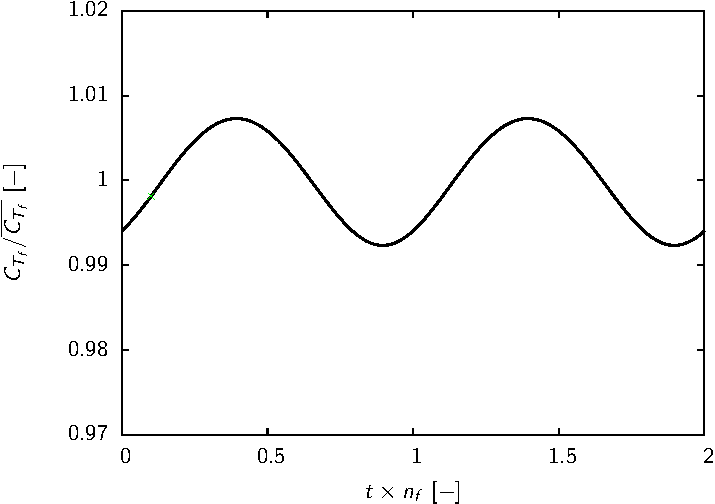
\includegraphics[width=.35\textwidth]{DREAM_HS_TSM_FORCES_INST_FRONT_PPT.pdf}}
  \subfigure[rear rotor]{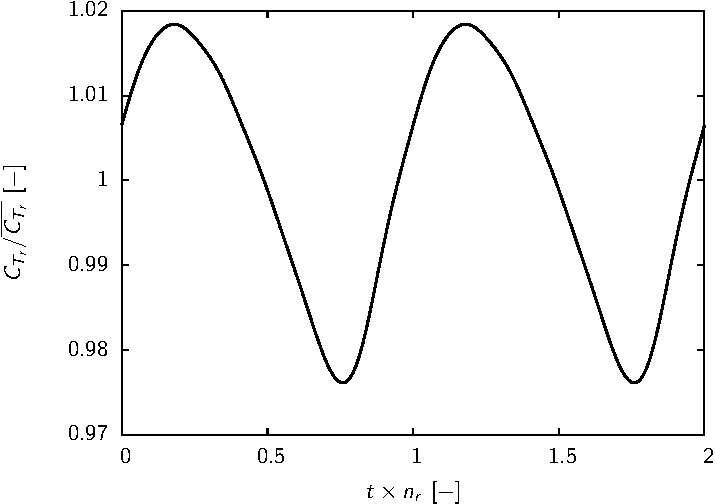
\includegraphics[width=.35\textwidth]{DREAM_HS_TSM_FORCES_INST_REAR_PPT.pdf}}
  \caption{High-speed isolated configuration: unsteadiness seen by the rotors.}
  \label{fig:dream_hs_hb_unst_coeff}
\end{figure}
The envelop of the unsteadiness is $\pm 1\%$ on the front rotor
and $\pm 2\%$ on the rear rotor. This has to be compared to 
the $\pm 3 \permil$ observed for the low-speed configuration.
The amplitude of unsteadiness is double on the rear rotor
meaning that the wake effects are much stronger than the
potential ones when considering the high-speed inflow condition.
The analysis of the shape of the unsteady thrust coefficient
reveals that it is close to a sine shape function for the front
rotor. It tends toward a Gaussian shape function for the rear rotor.

\subsection{Two-dimensional results: harmonic blade response}
\label{sub:dream_hs_hb_blade_response}

To further analyze the unsteadinesses perceived by both rotors,
a discrete Fourier transform of the first harmonic pressure
of the opposite blade passing frequency is shown in 
Fig.~\ref{fig:dream_hs_hb_blade_response}. Note that the
scale is different for the front and the rear rotor.
\begin{figure}[htp]
 \ra{1.3} \centering
 \begin{tabular}{cccc}
    \multicolumn{2}{c}{\includegraphics[width=0.3\textwidth]{dream_HS_blade_resp_scale_H01_front.pdf}} &
    \multicolumn{2}{c}{\includegraphics[width=0.3\textwidth]{dream_HS_blade_resp_scale_H01_rear.pdf}} \\
    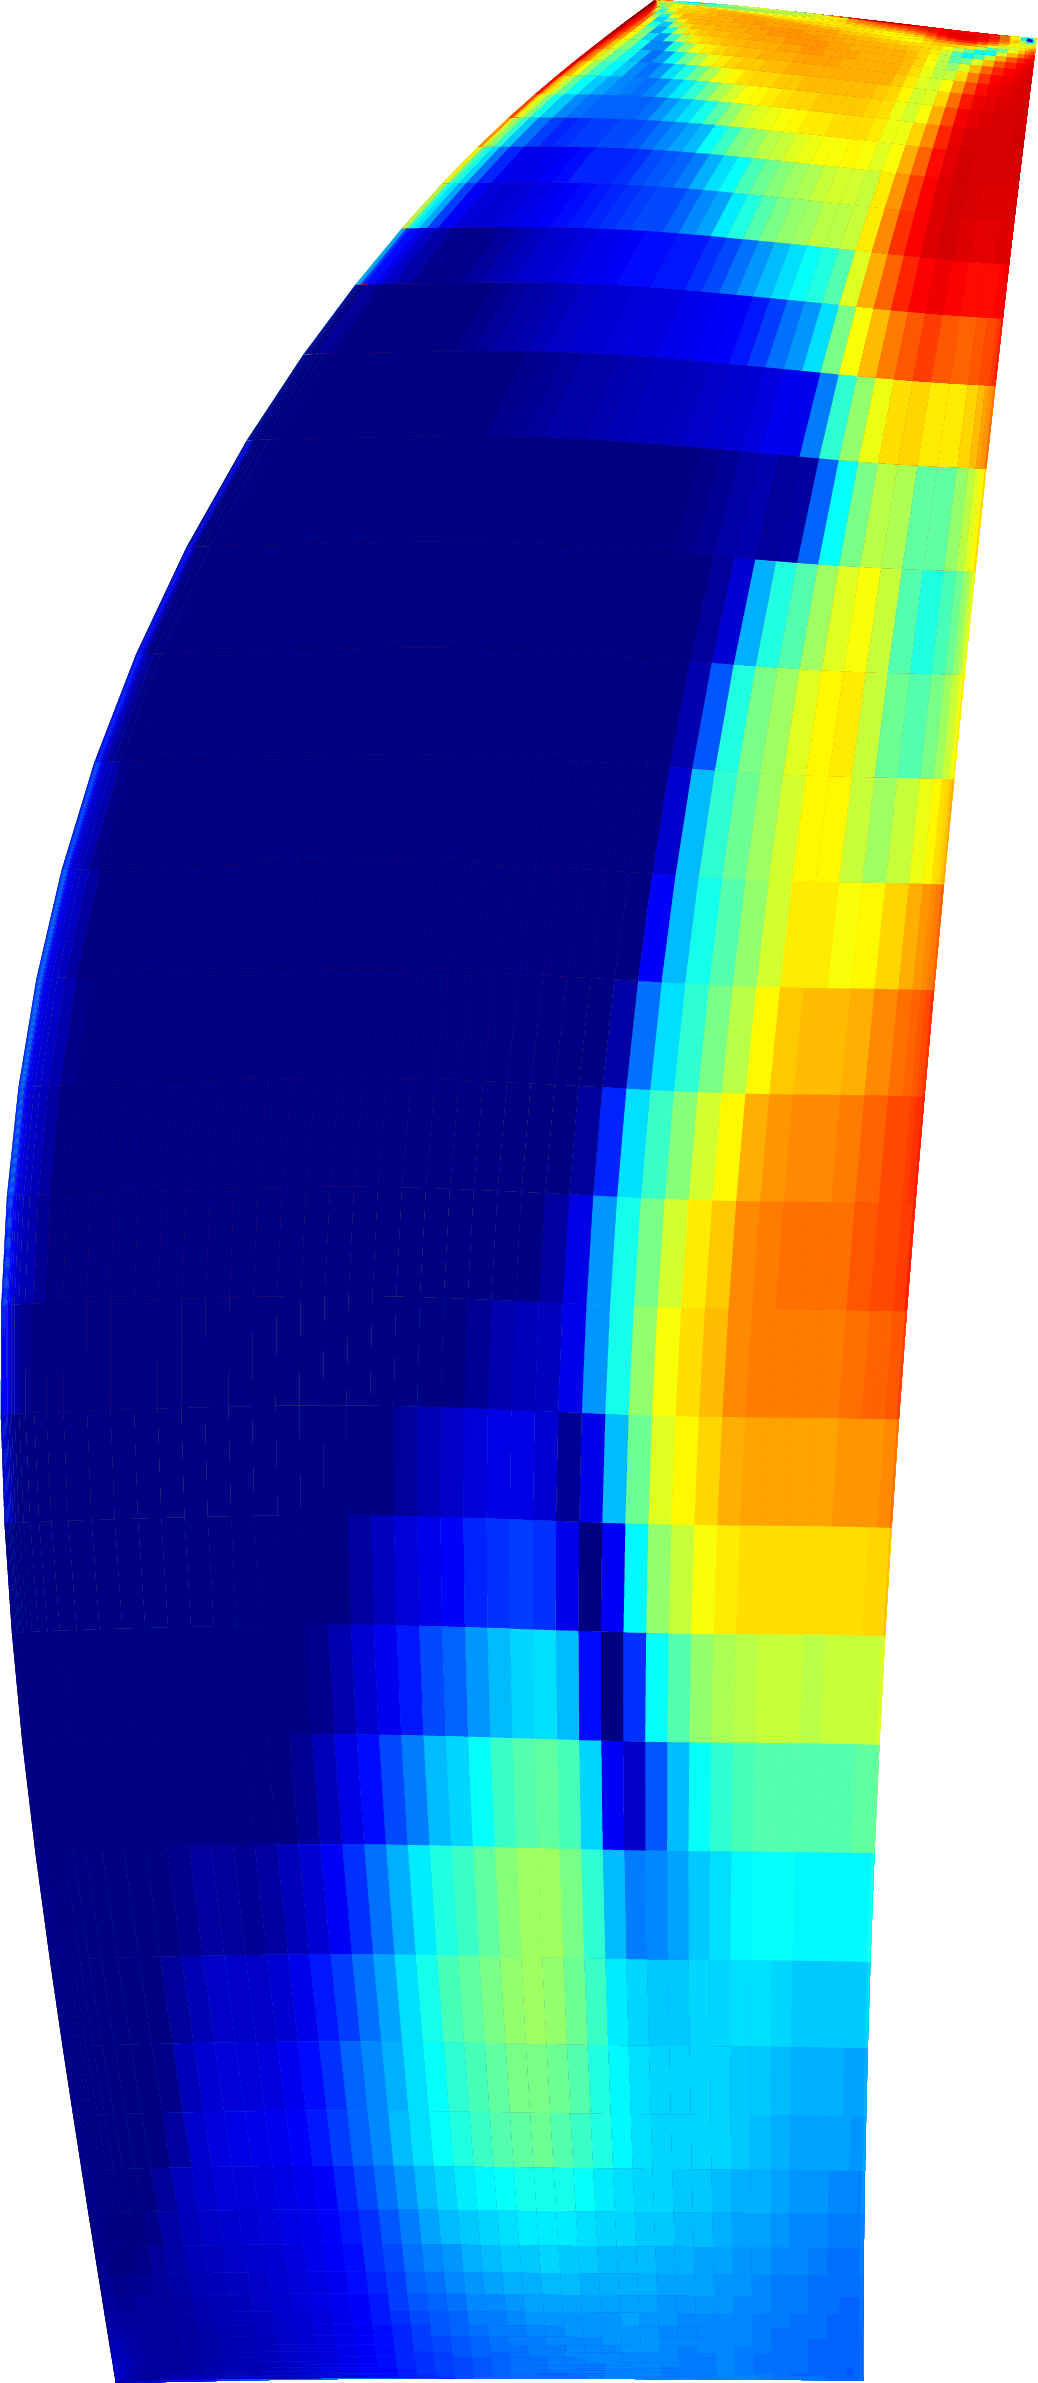
\includegraphics[width=0.15\textwidth]{DREAM_HS_TSM_N7_roe2_sa_blade_response_front_H01_SS.png}
    & 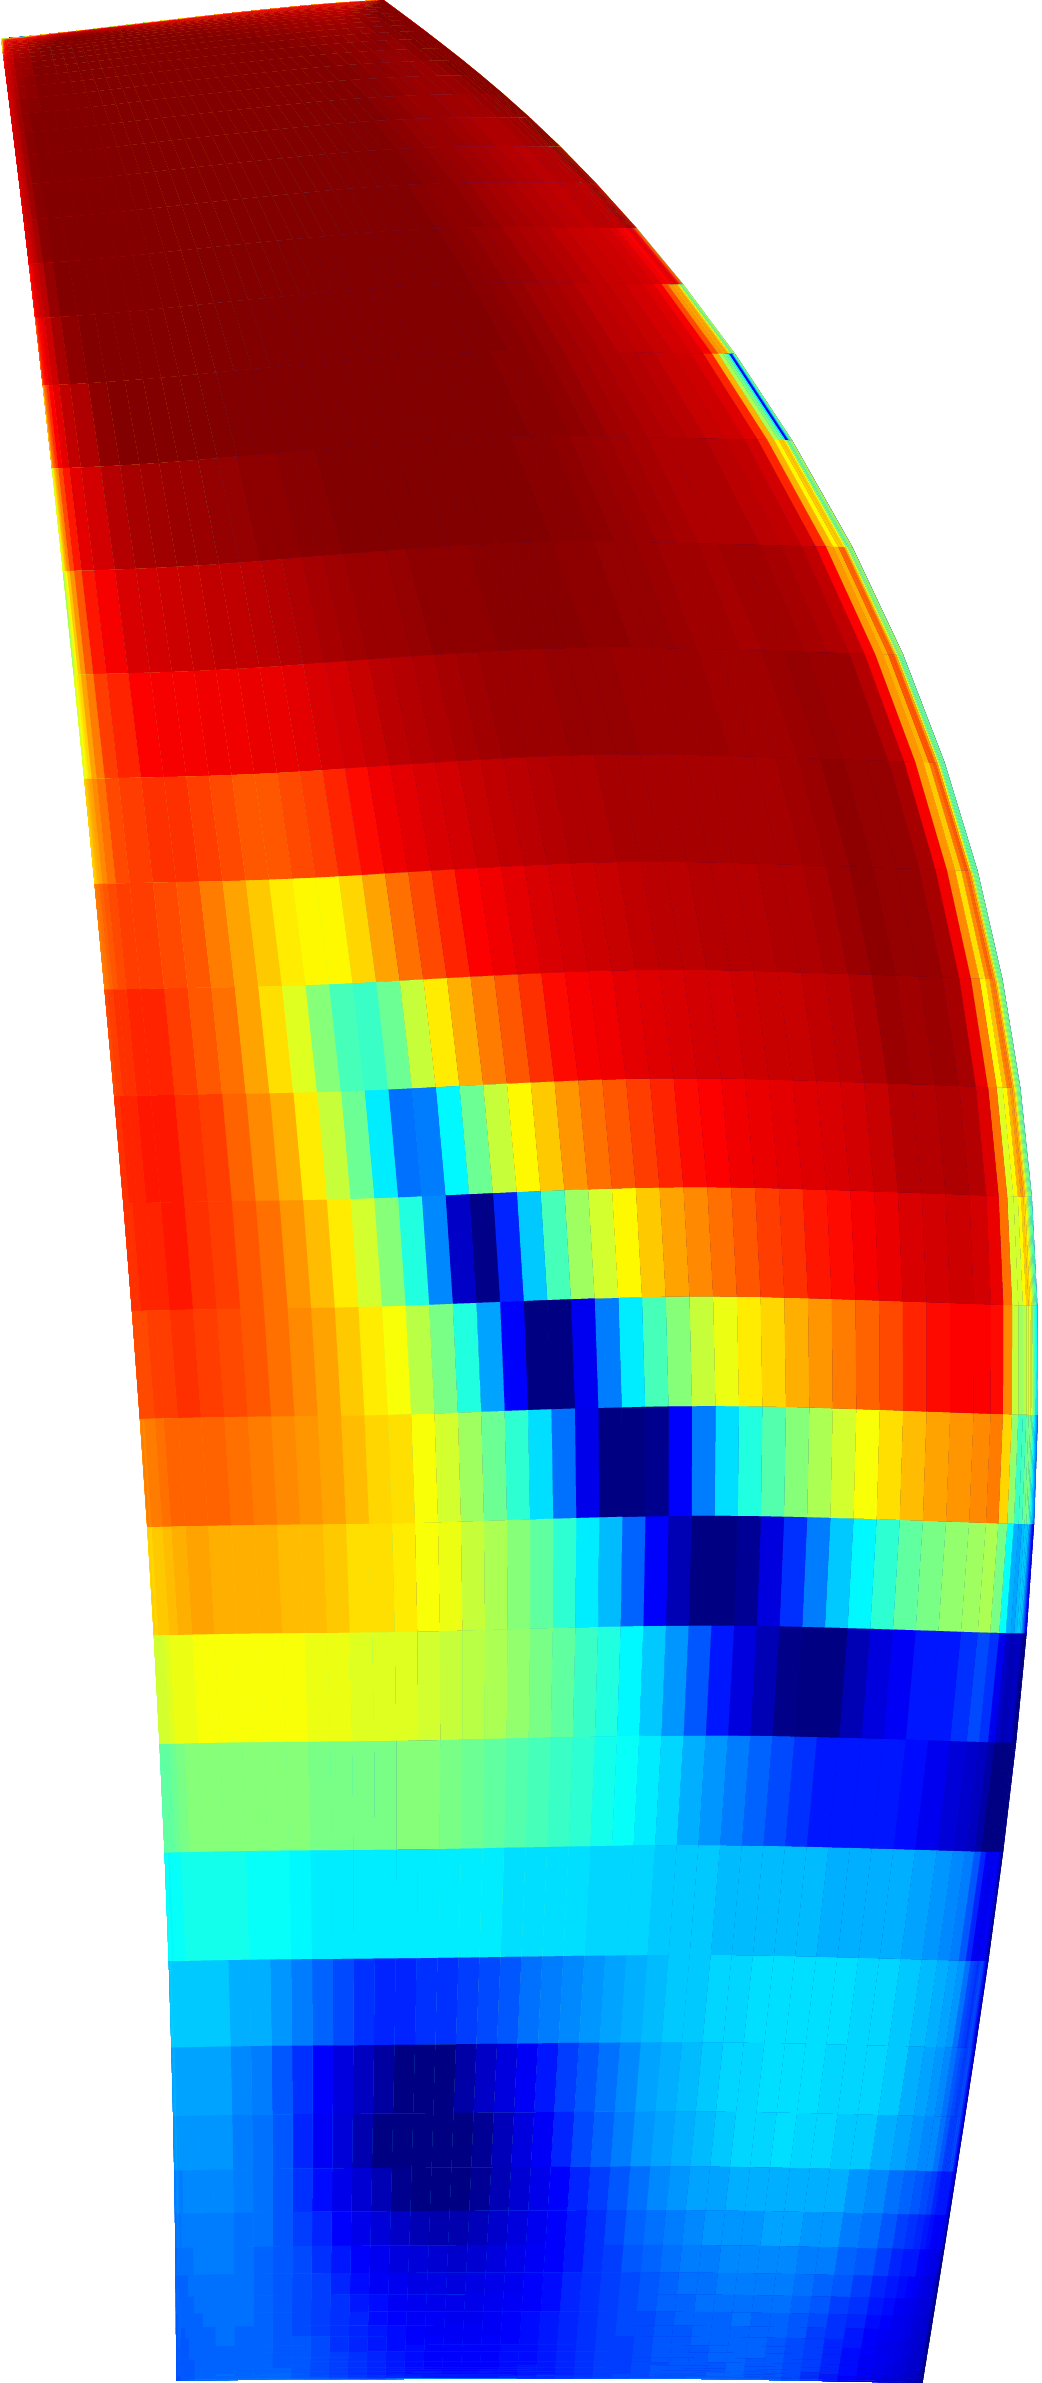
\includegraphics[width=0.15\textwidth]{DREAM_HS_TSM_N7_roe2_sa_blade_response_front_H01_PS.png}
    & 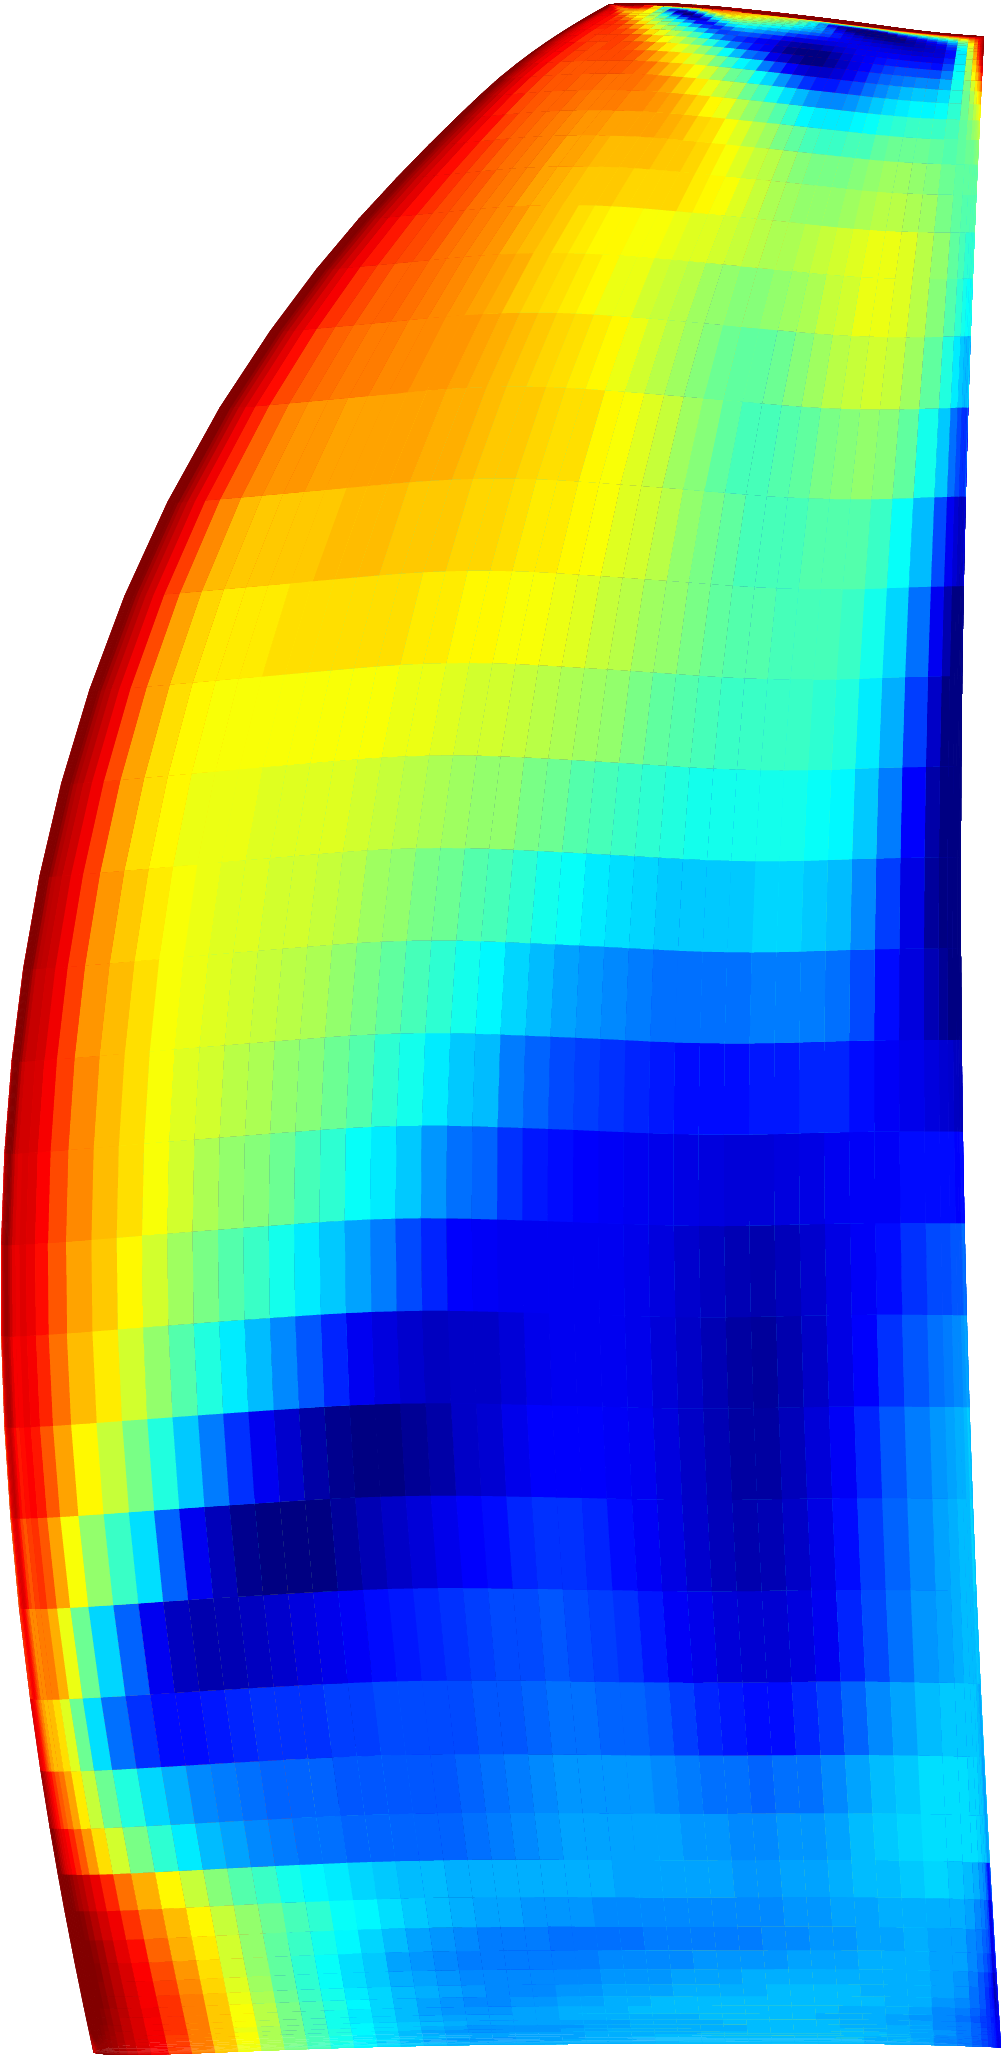
\includegraphics[width=0.15\textwidth]{DREAM_HS_TSM_N7_roe2_sa_blade_response_rear_H01_PS.png}
    & 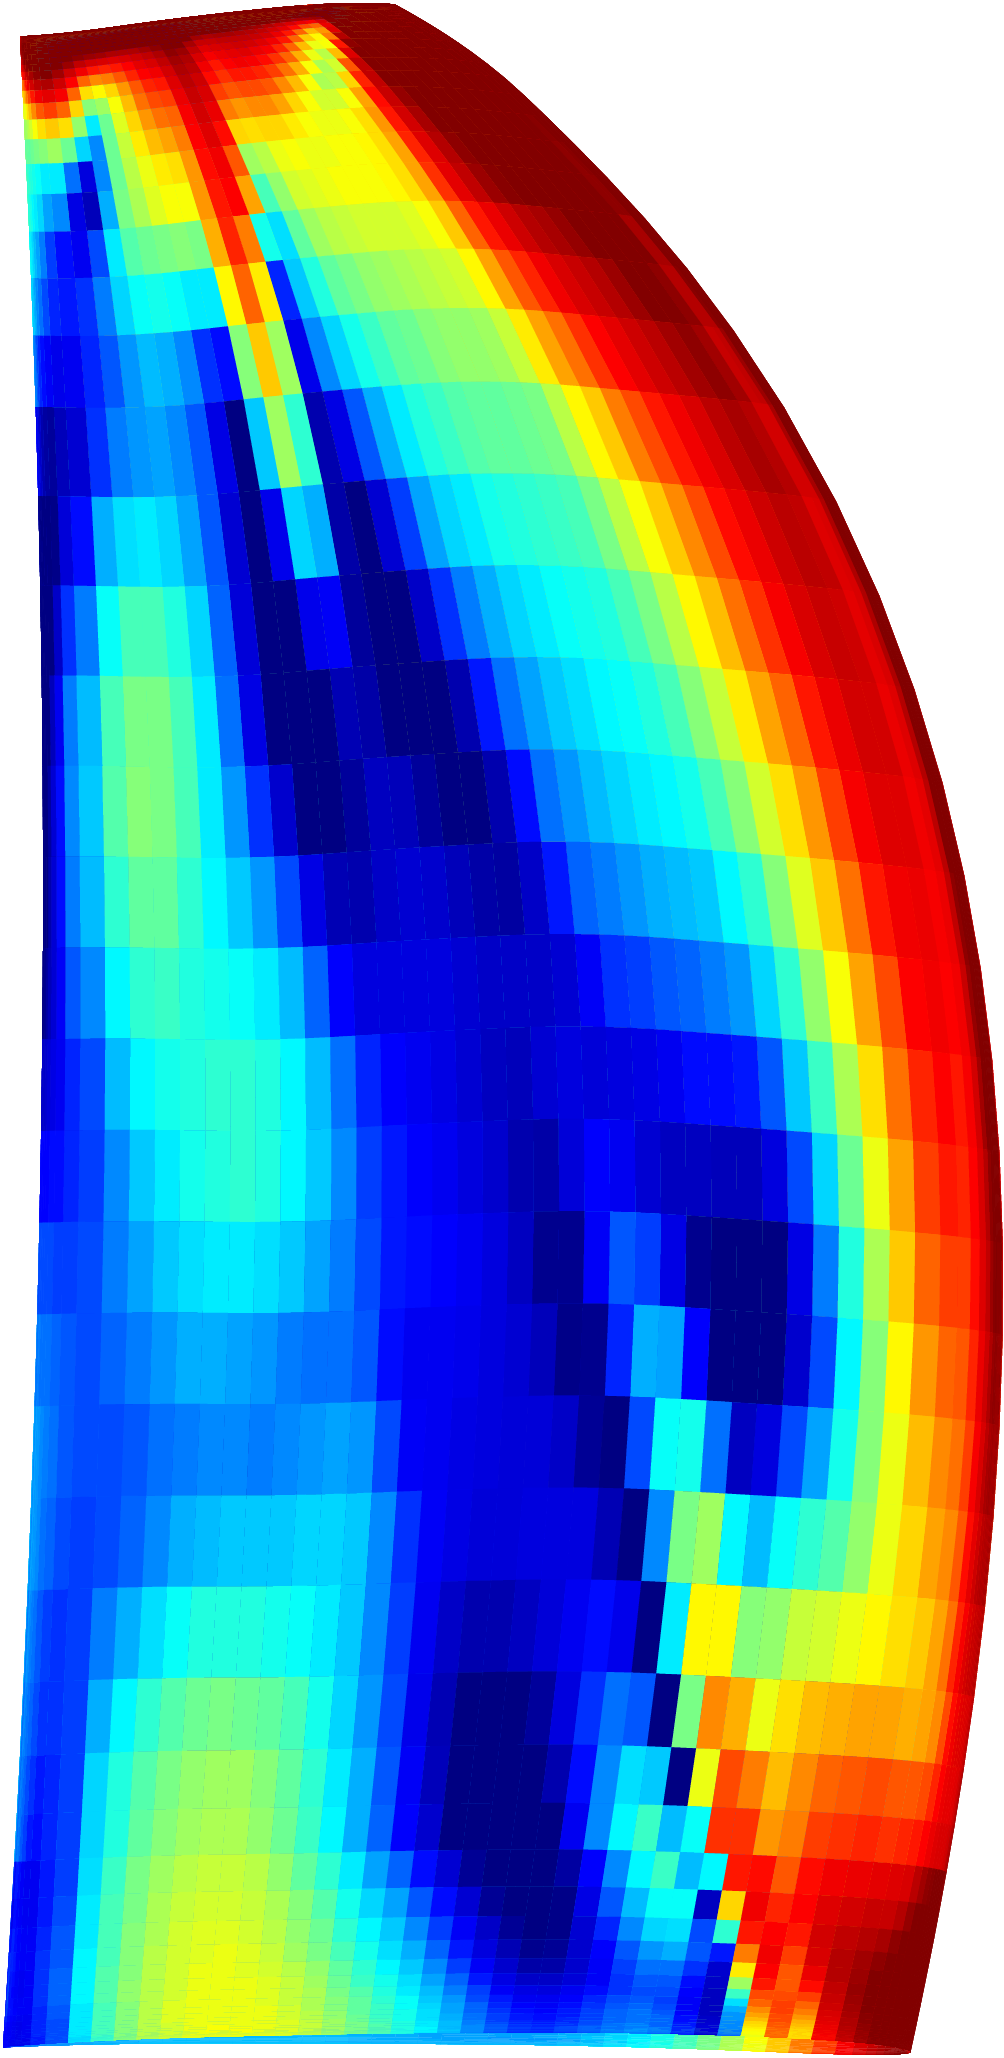
\includegraphics[width=0.15\textwidth]{DREAM_HS_TSM_N7_roe2_sa_blade_response_rear_H01_SS.png} \\
    \multicolumn{2}{c}{\emph{Front rotor blade}}
    & \multicolumn{2}{c}{\emph{Rear rotor blade}} \\
    suction side & pressure side & pressure side & suction side
 \end{tabular}
 \caption{High-speed isolated configuration: harmonic response of the front
 rotor blades.}
 \label{fig:dream_hs_hb_blade_response}
\end{figure}

The maximum amplitude for the front rotor blade 
is observed at the tip of the pressure side. This is consistent
with the observation made on the low-speed configuration, where
the suction side was more exposed to pressure variations as
the pressure side was shield by the blade angle of attack.
The pressure side is not only shield by the blade angle
of attack but also by the shock that forms around 
$x/c \approx 0.7$ for relative span greater than $40\%$,
as mentioned in Sec.~\ref{sub:dream_hs_blades}. For
relative span smaller than $40\%$, the shock is closer the
leading edge, hence the pressure unsteadiness that goes
upstream. On the tip of the front rotor blade,
a tip vortex is formed that leaves the blades from the pressure
side to the suction side. This tip vortex increases 
the pressure on the suction side, alleviating the formation
of a shock. Therefore, as near the hub, the pressure variations
can go upstream and thus affects the entire tip of the blade.

\subsection{Two-dimensional results: axial cuts}
\label{sub:dream_hs_hb_axial_cuts}

\begin{figure}[htp]
 \ra{1.3} \centering
 \begin{tabular}{rcc}
   & steady
   & HB $N=4$ \\
   \rotatebox{90}{\qquad\qquad\qquad $P3$} & 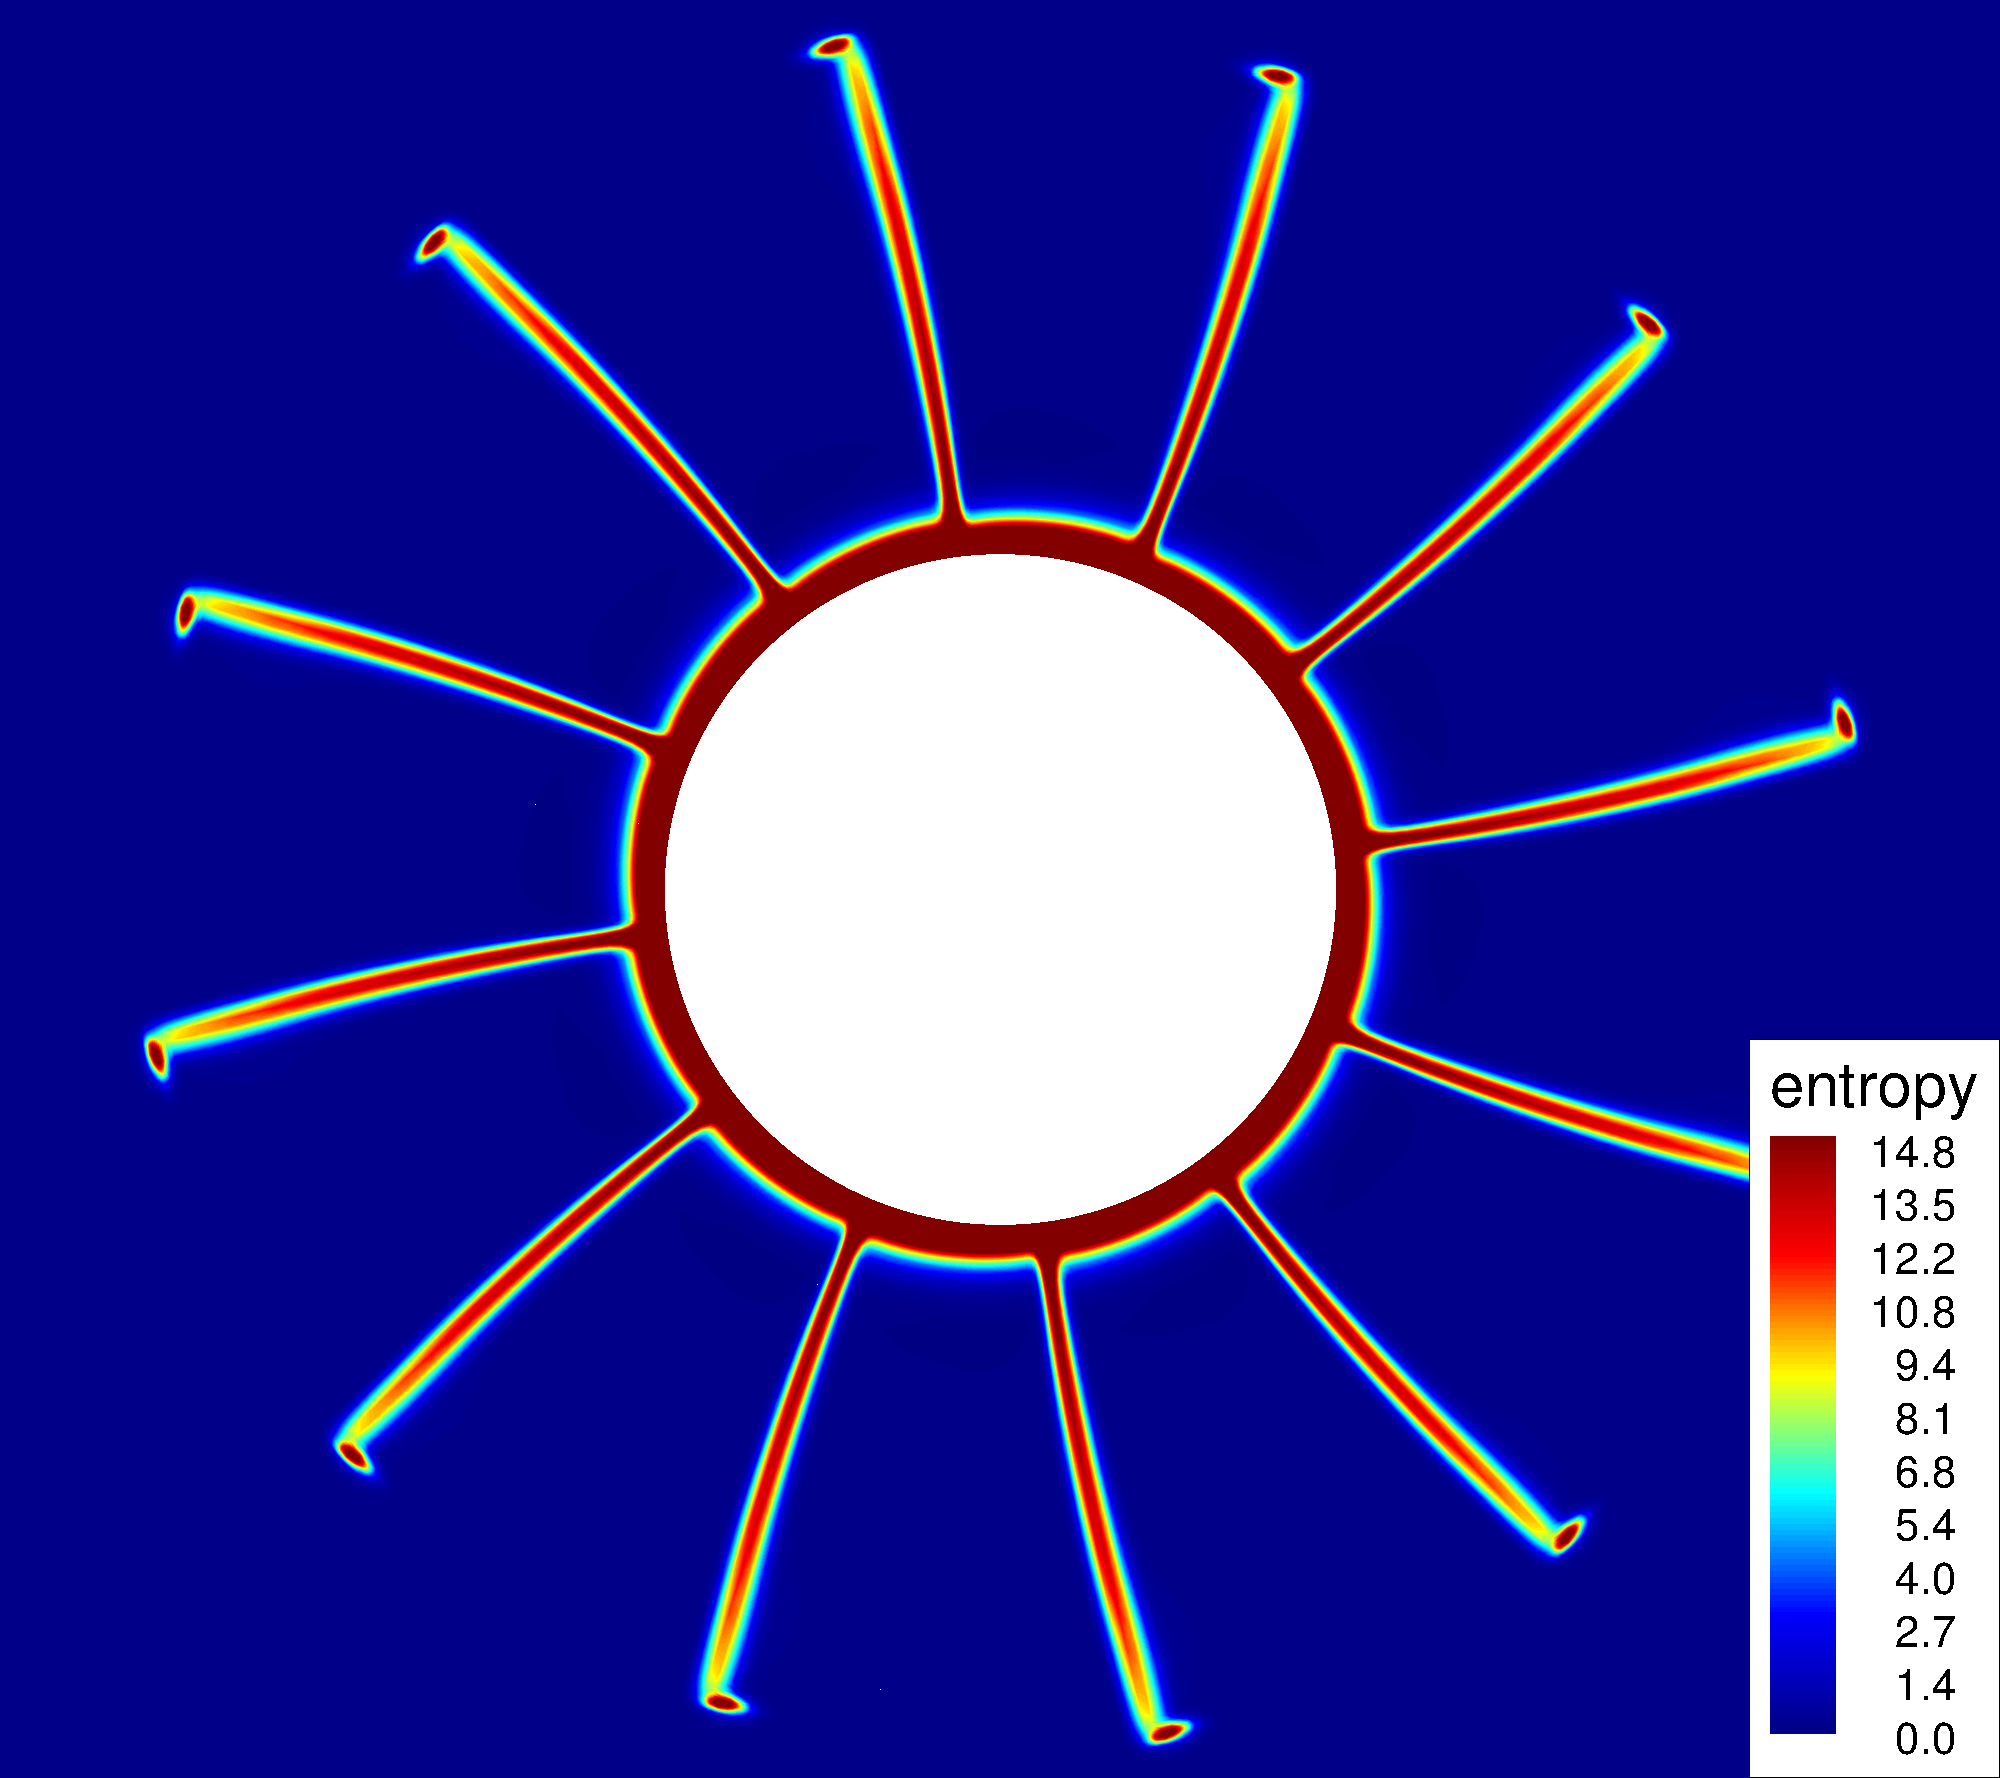
\includegraphics[width=.35\textwidth]{DREAM_HS_RANS_roe2_sa_slice_x_front_1_entropy.png}
   & 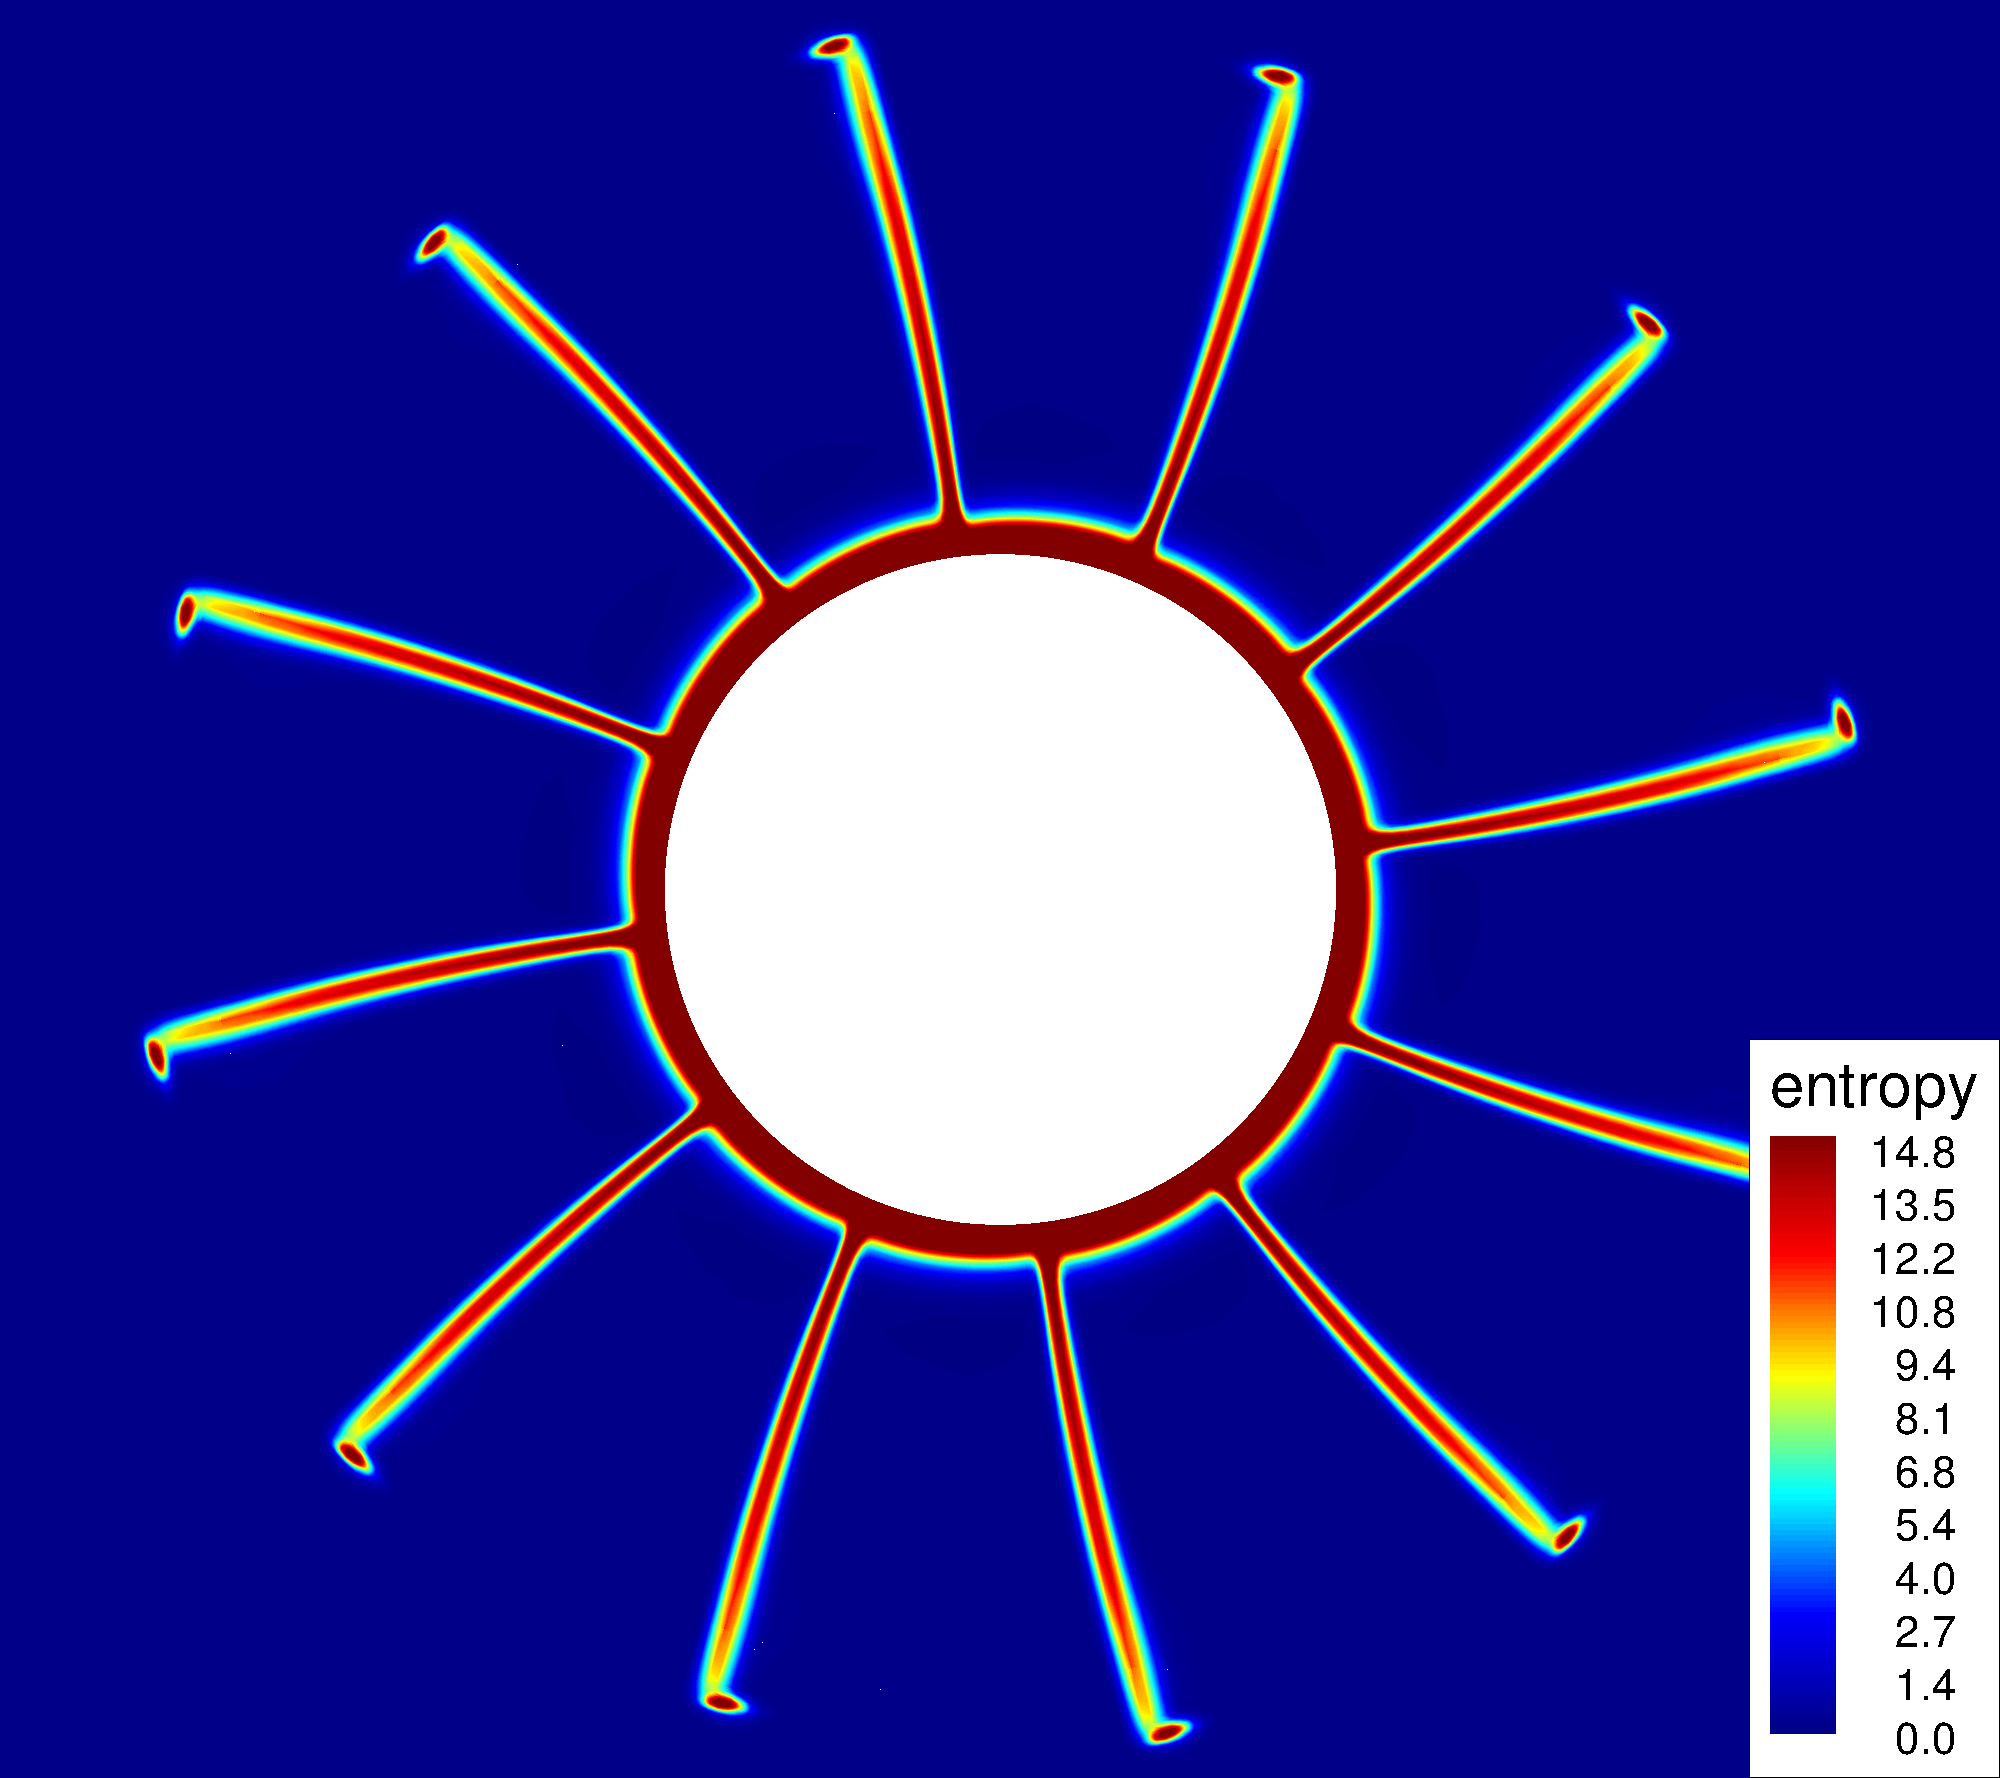
\includegraphics[width=.35\textwidth]{DREAM_HS_TSM_N7_roe2_sa_slice_x_front_1_entropy.png} \\
   \rotatebox{90}{\qquad\qquad\qquad $P4$} & 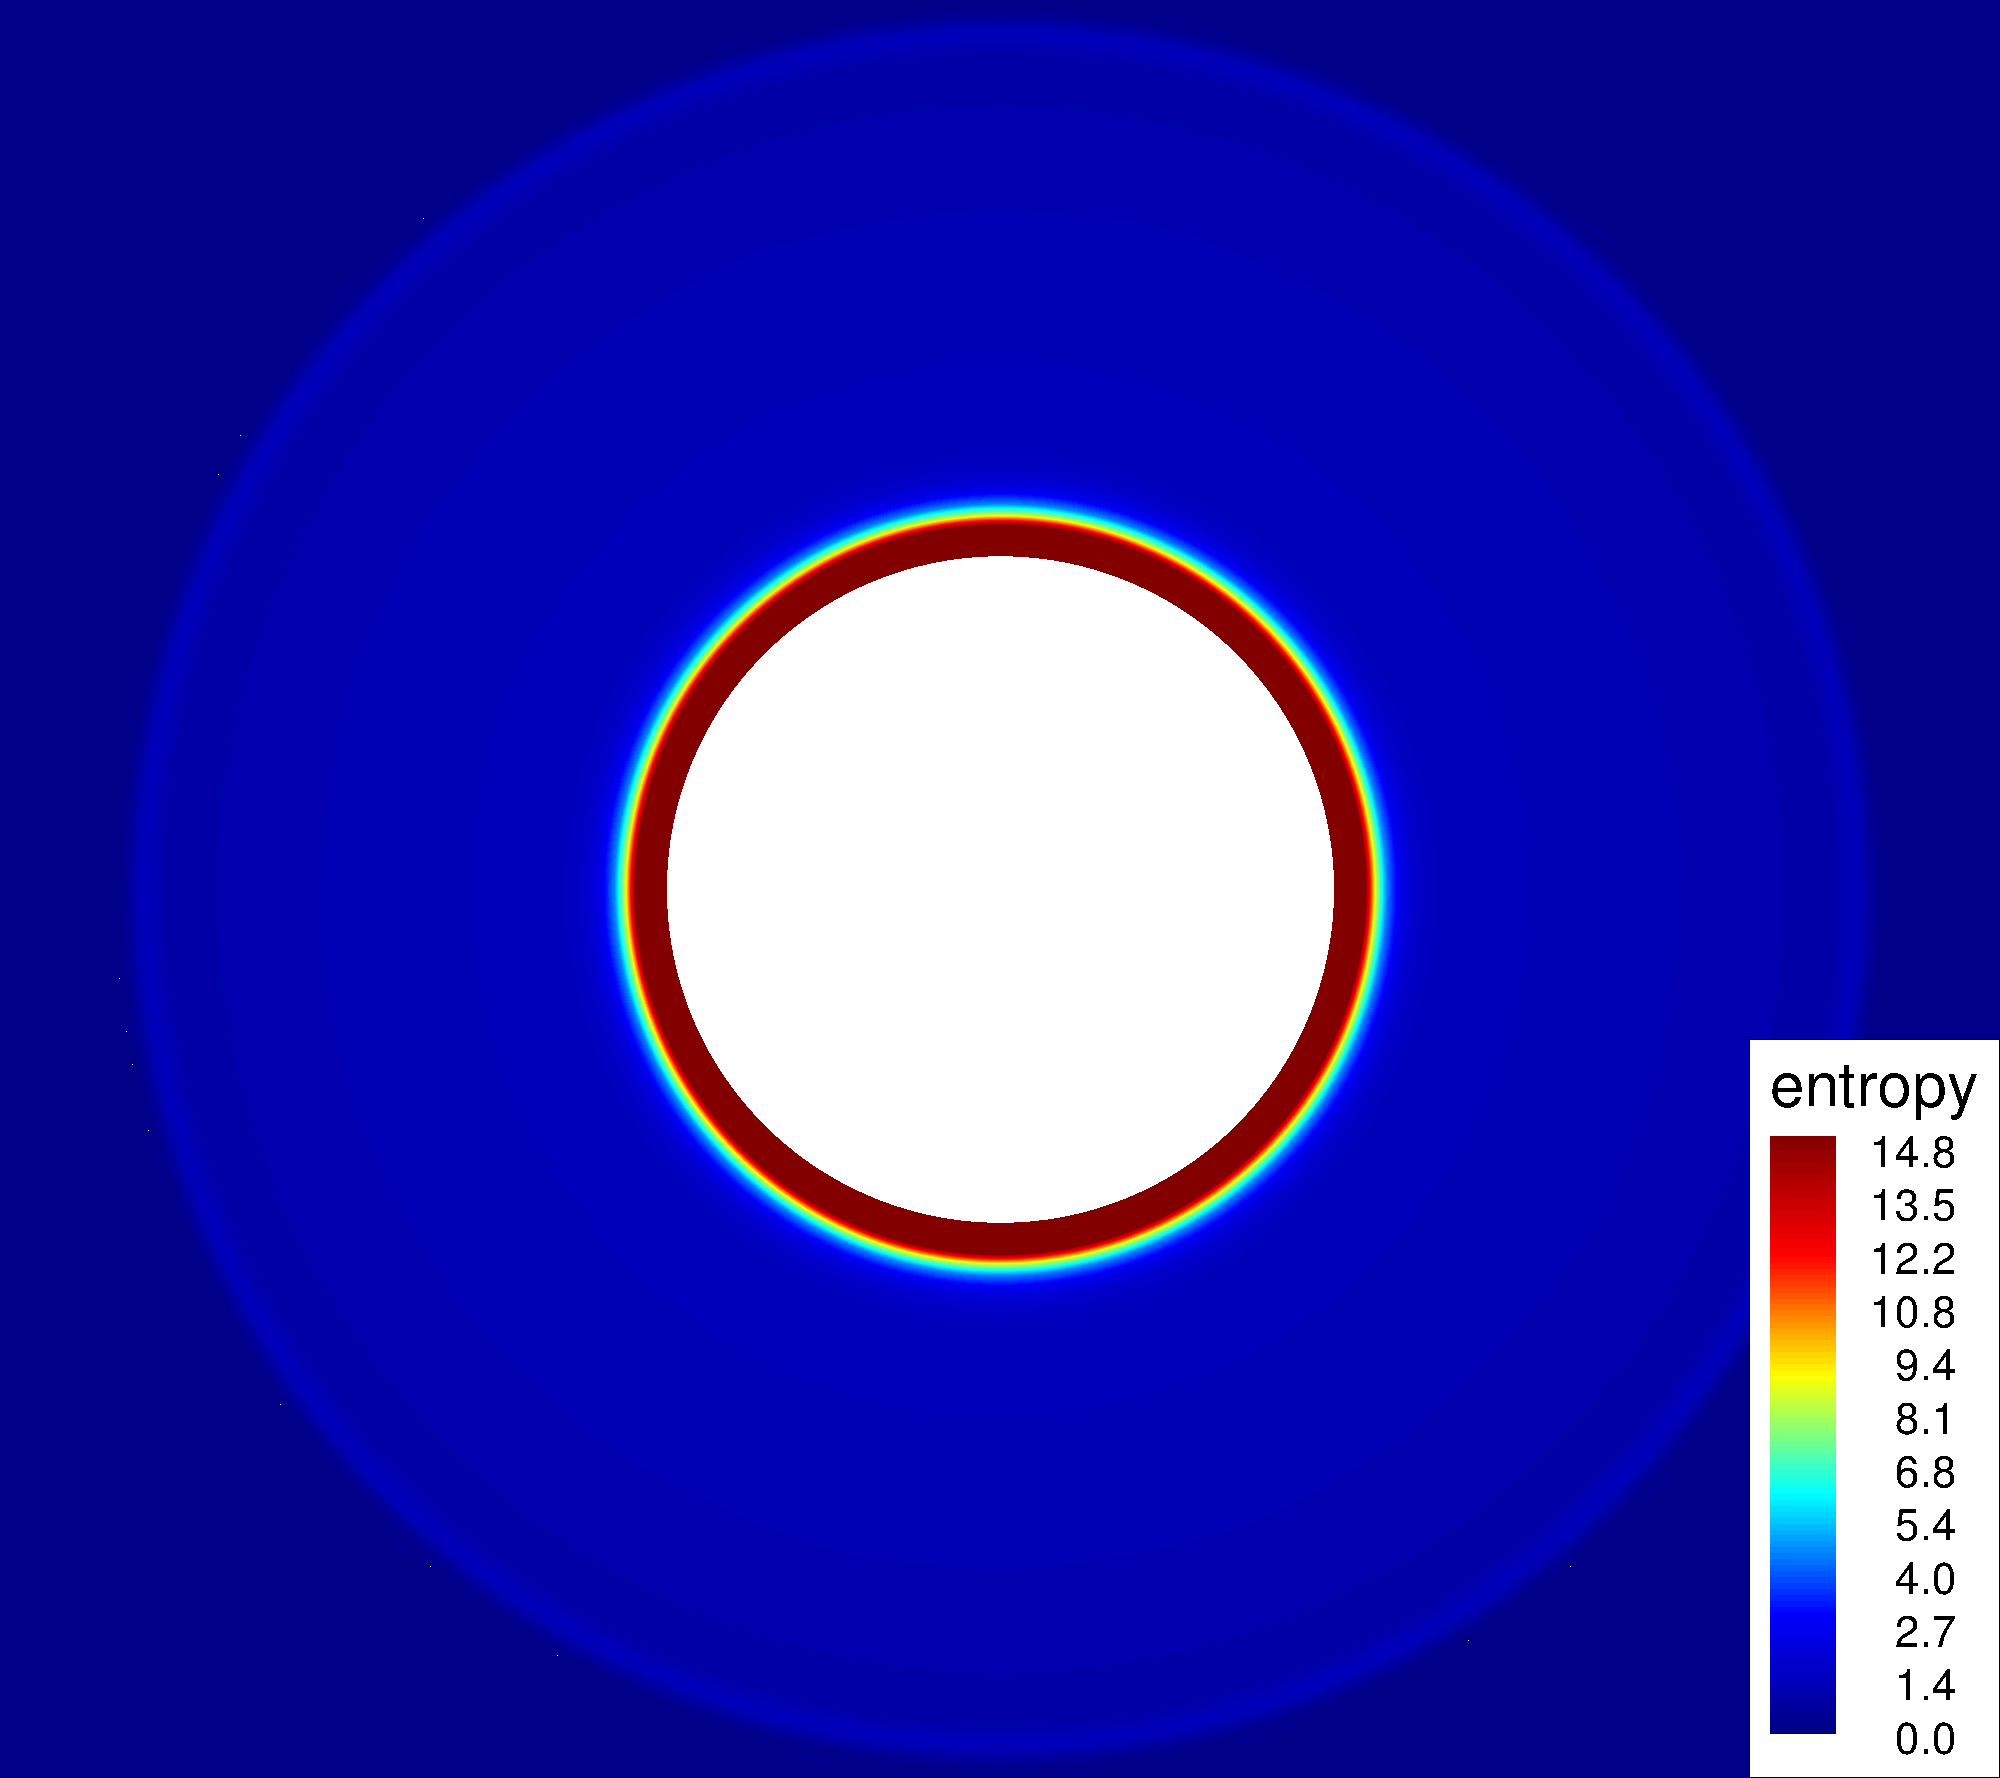
\includegraphics[width=.35\textwidth]{DREAM_HS_RANS_roe2_sa_slice_x_rear_0_entropy.png}
   & 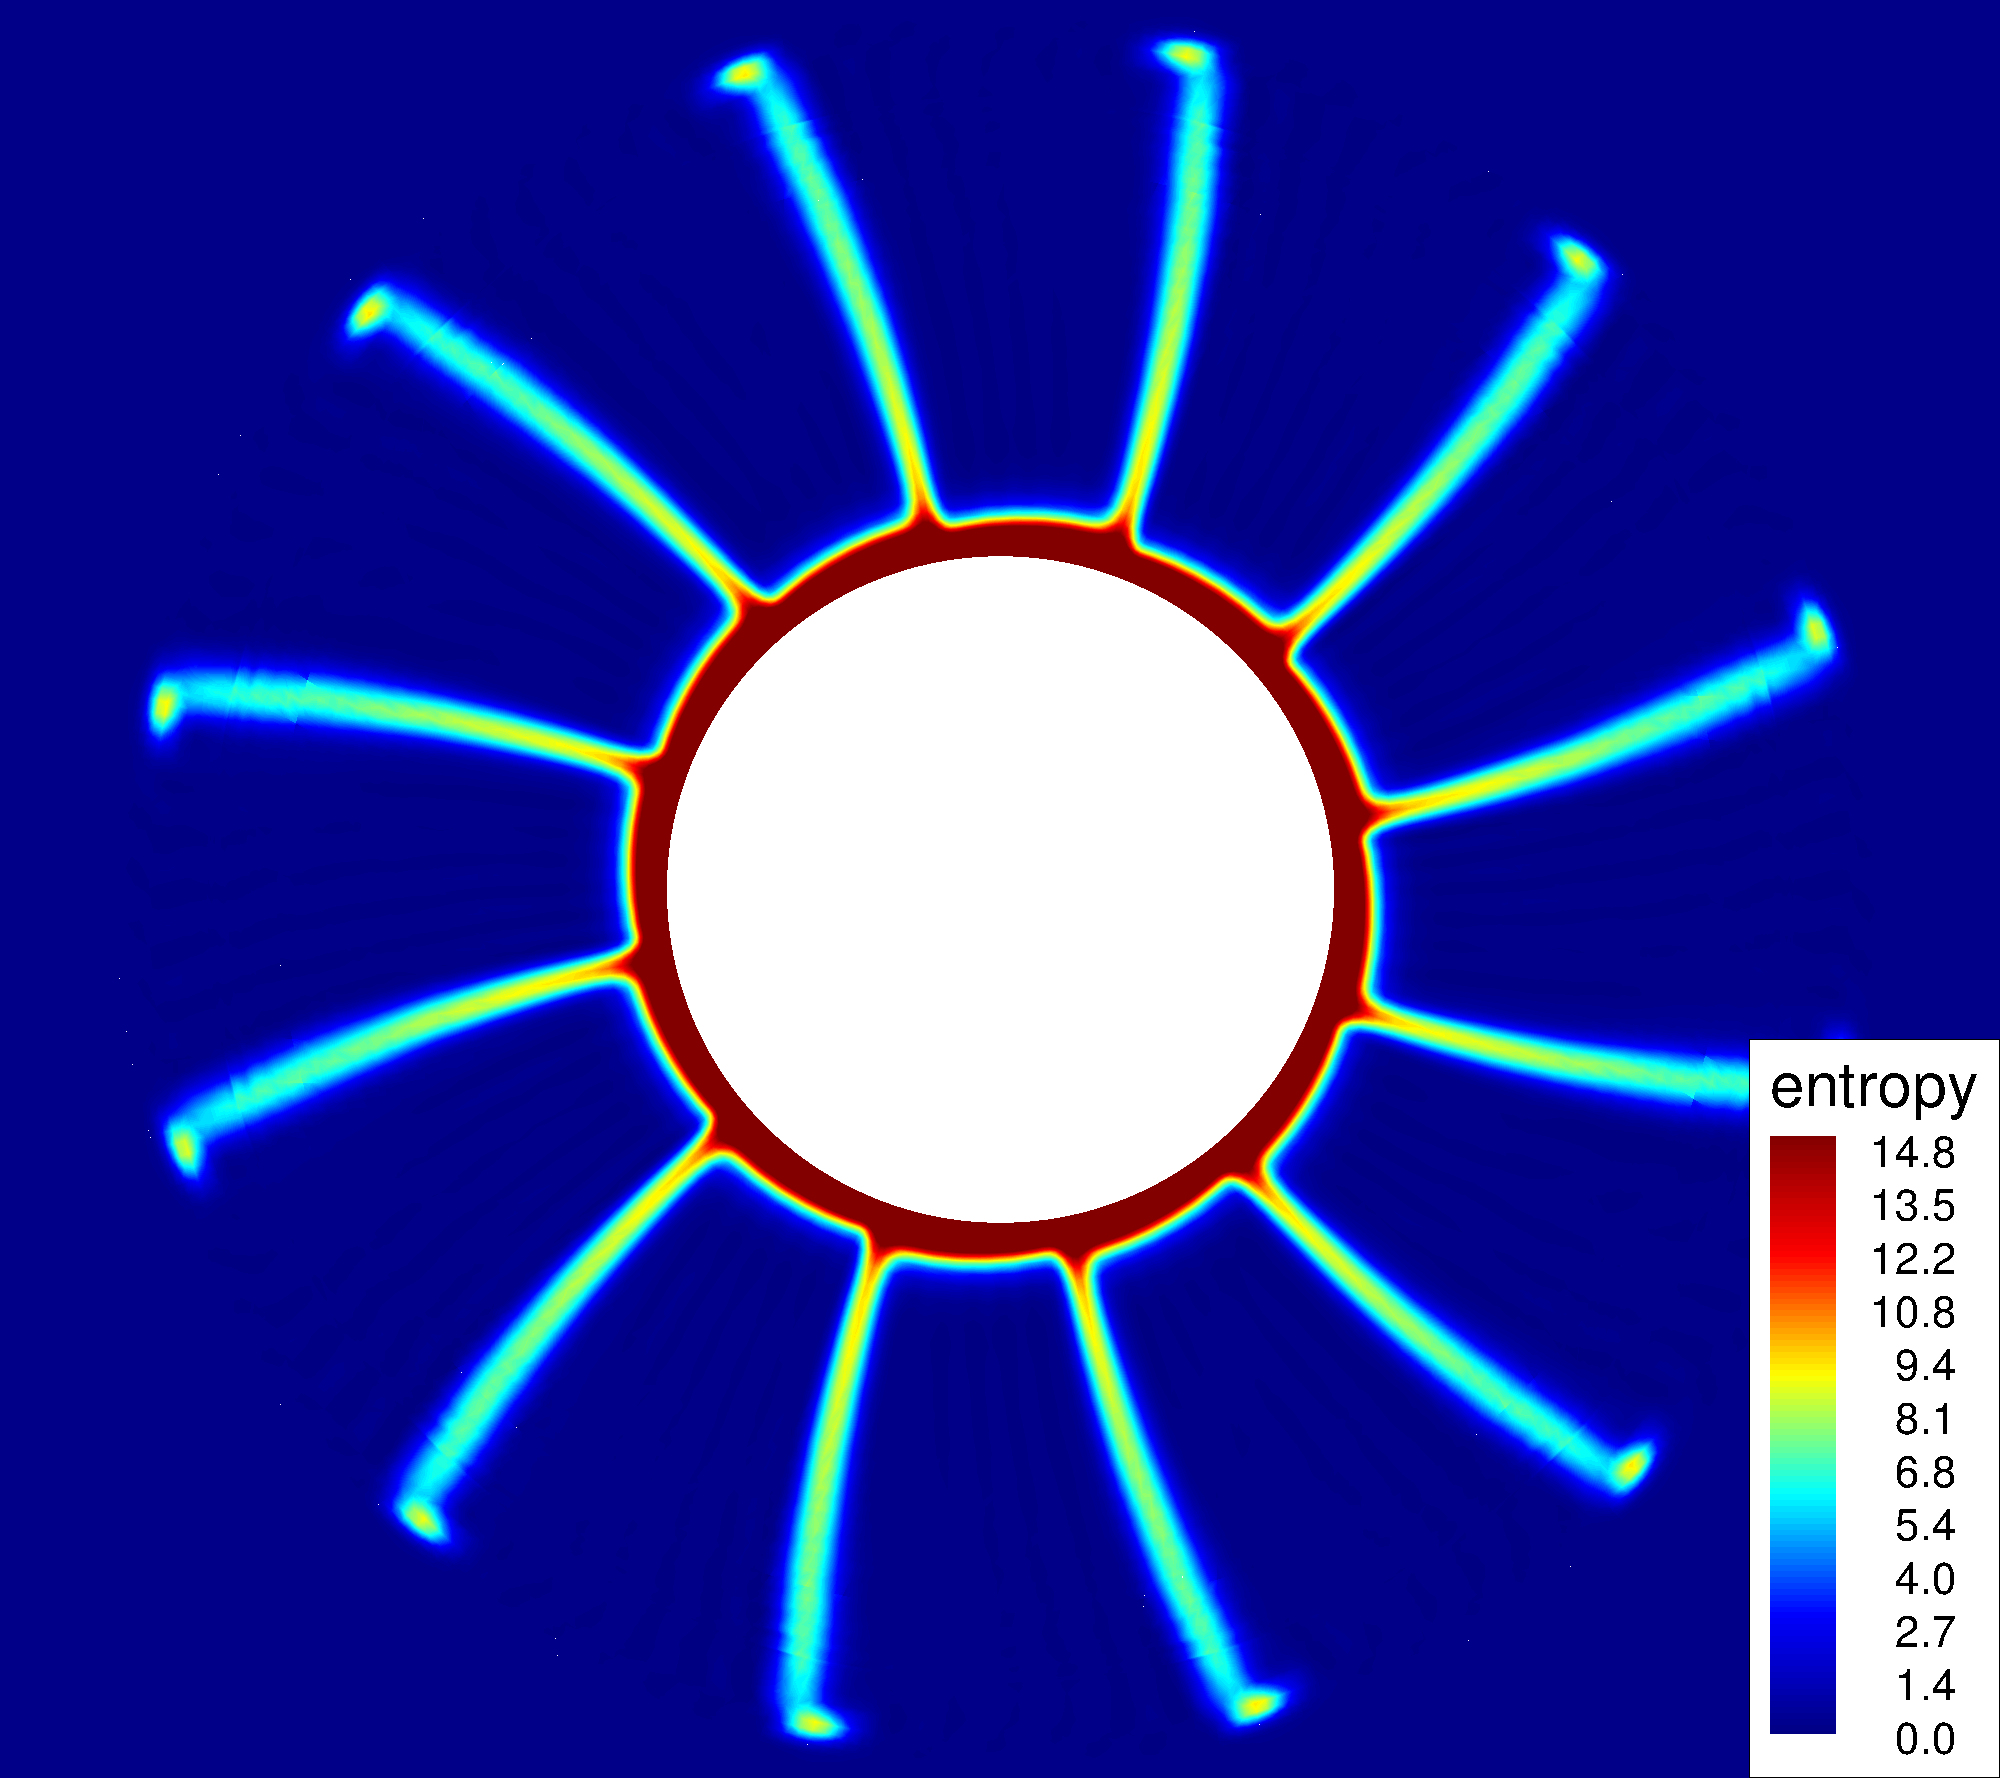
\includegraphics[width=.35\textwidth]{DREAM_HS_TSM_N7_roe2_sa_slice_x_rear_0_entropy.png} \\
   \rotatebox{90}{\qquad\qquad\qquad $P5$} & 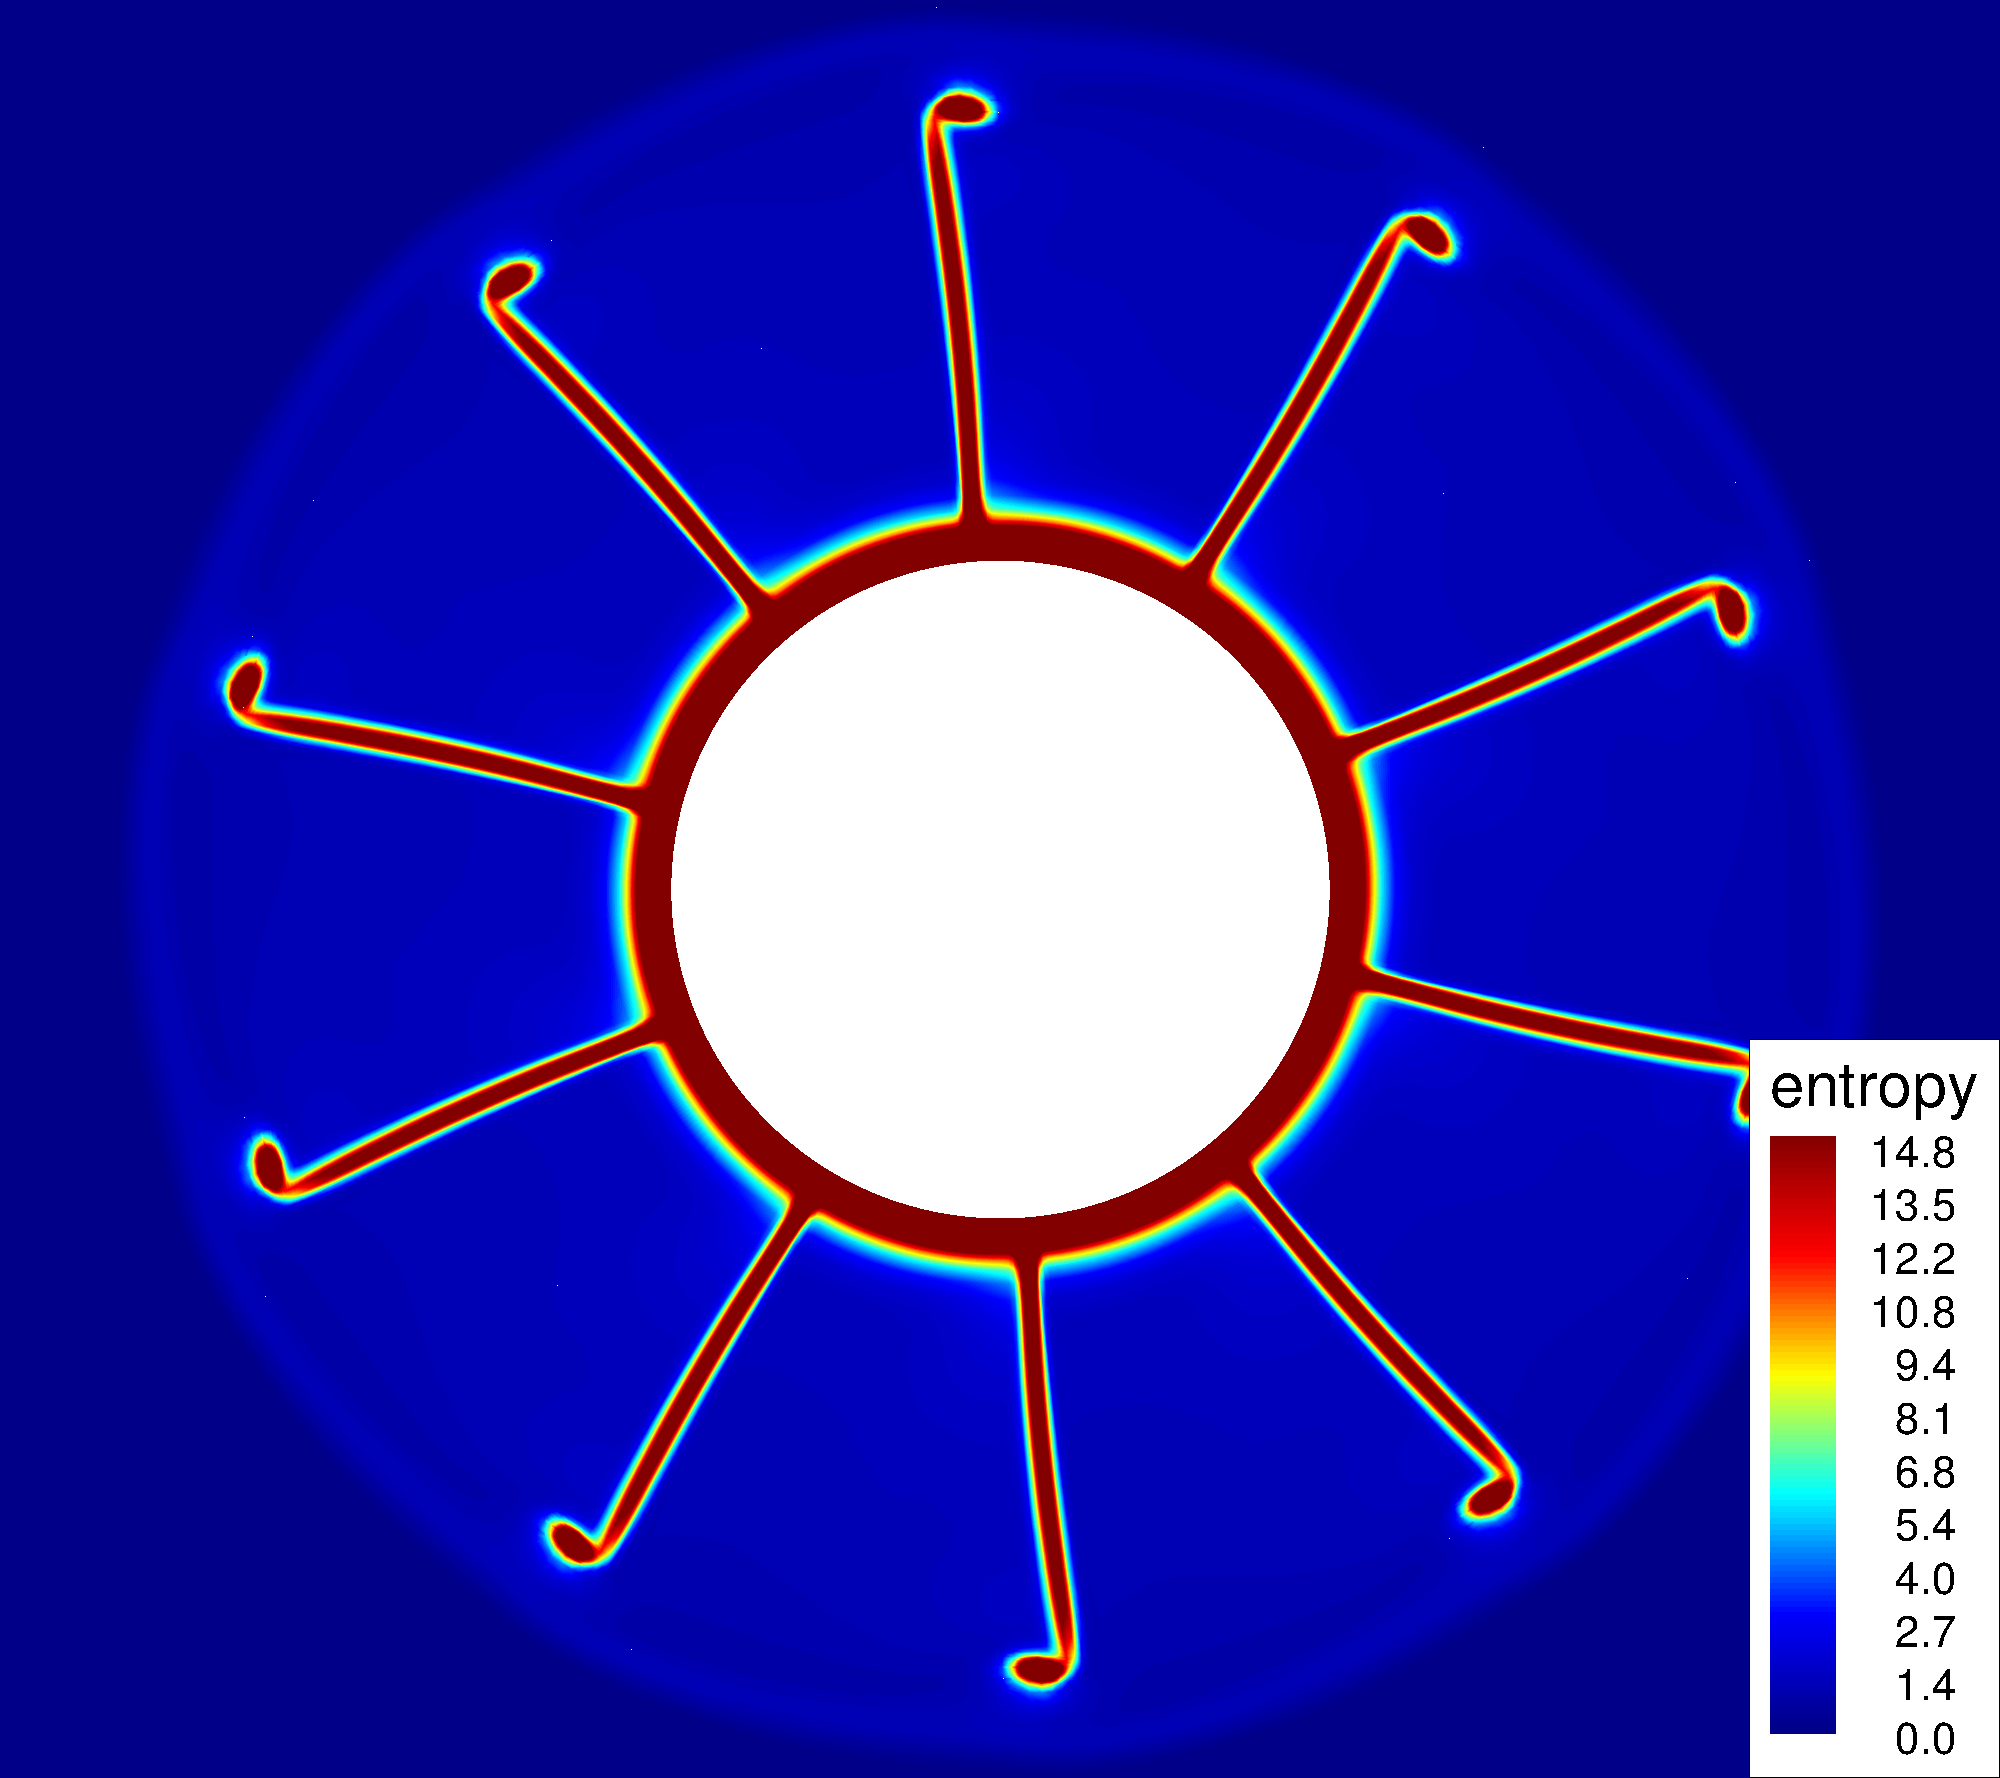
\includegraphics[width=.35\textwidth]{DREAM_HS_RANS_roe2_sa_slice_x_rear_1_entropy.png}
   & 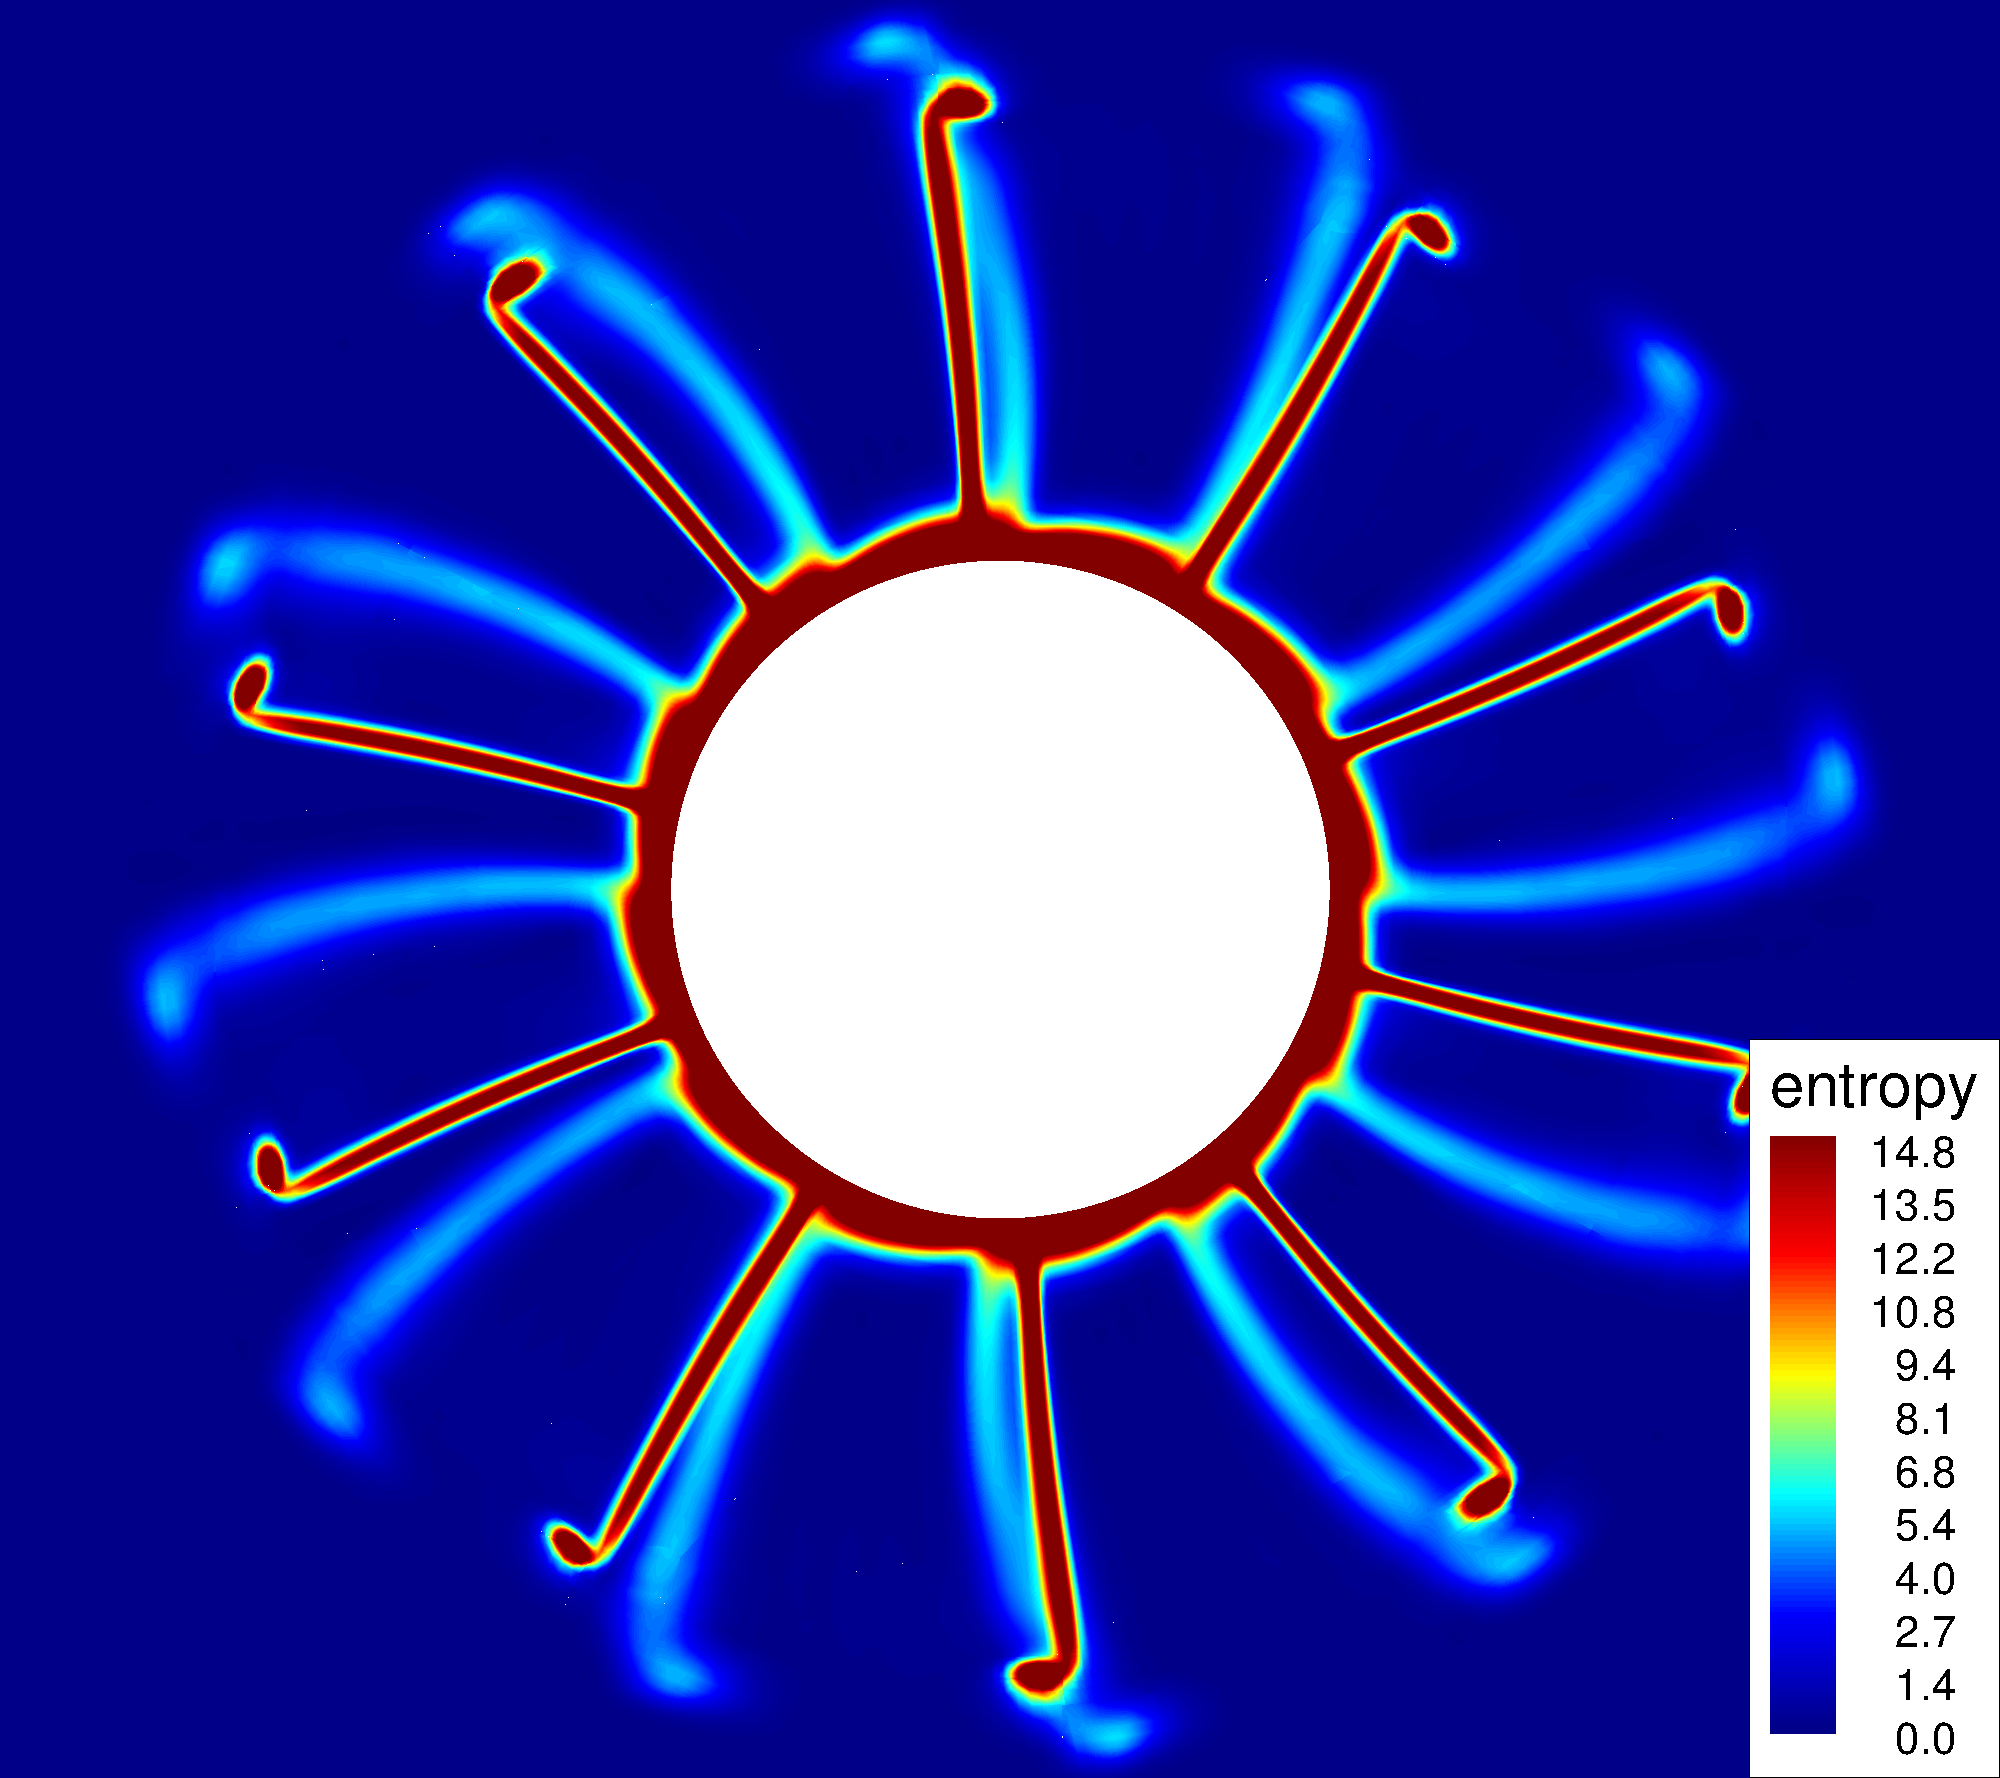
\includegraphics[width=.35\textwidth]{DREAM_HS_TSM_N7_roe2_sa_slice_x_rear_1_entropy.png} \\
   \rotatebox{90}{\qquad\qquad\qquad $P6$} & 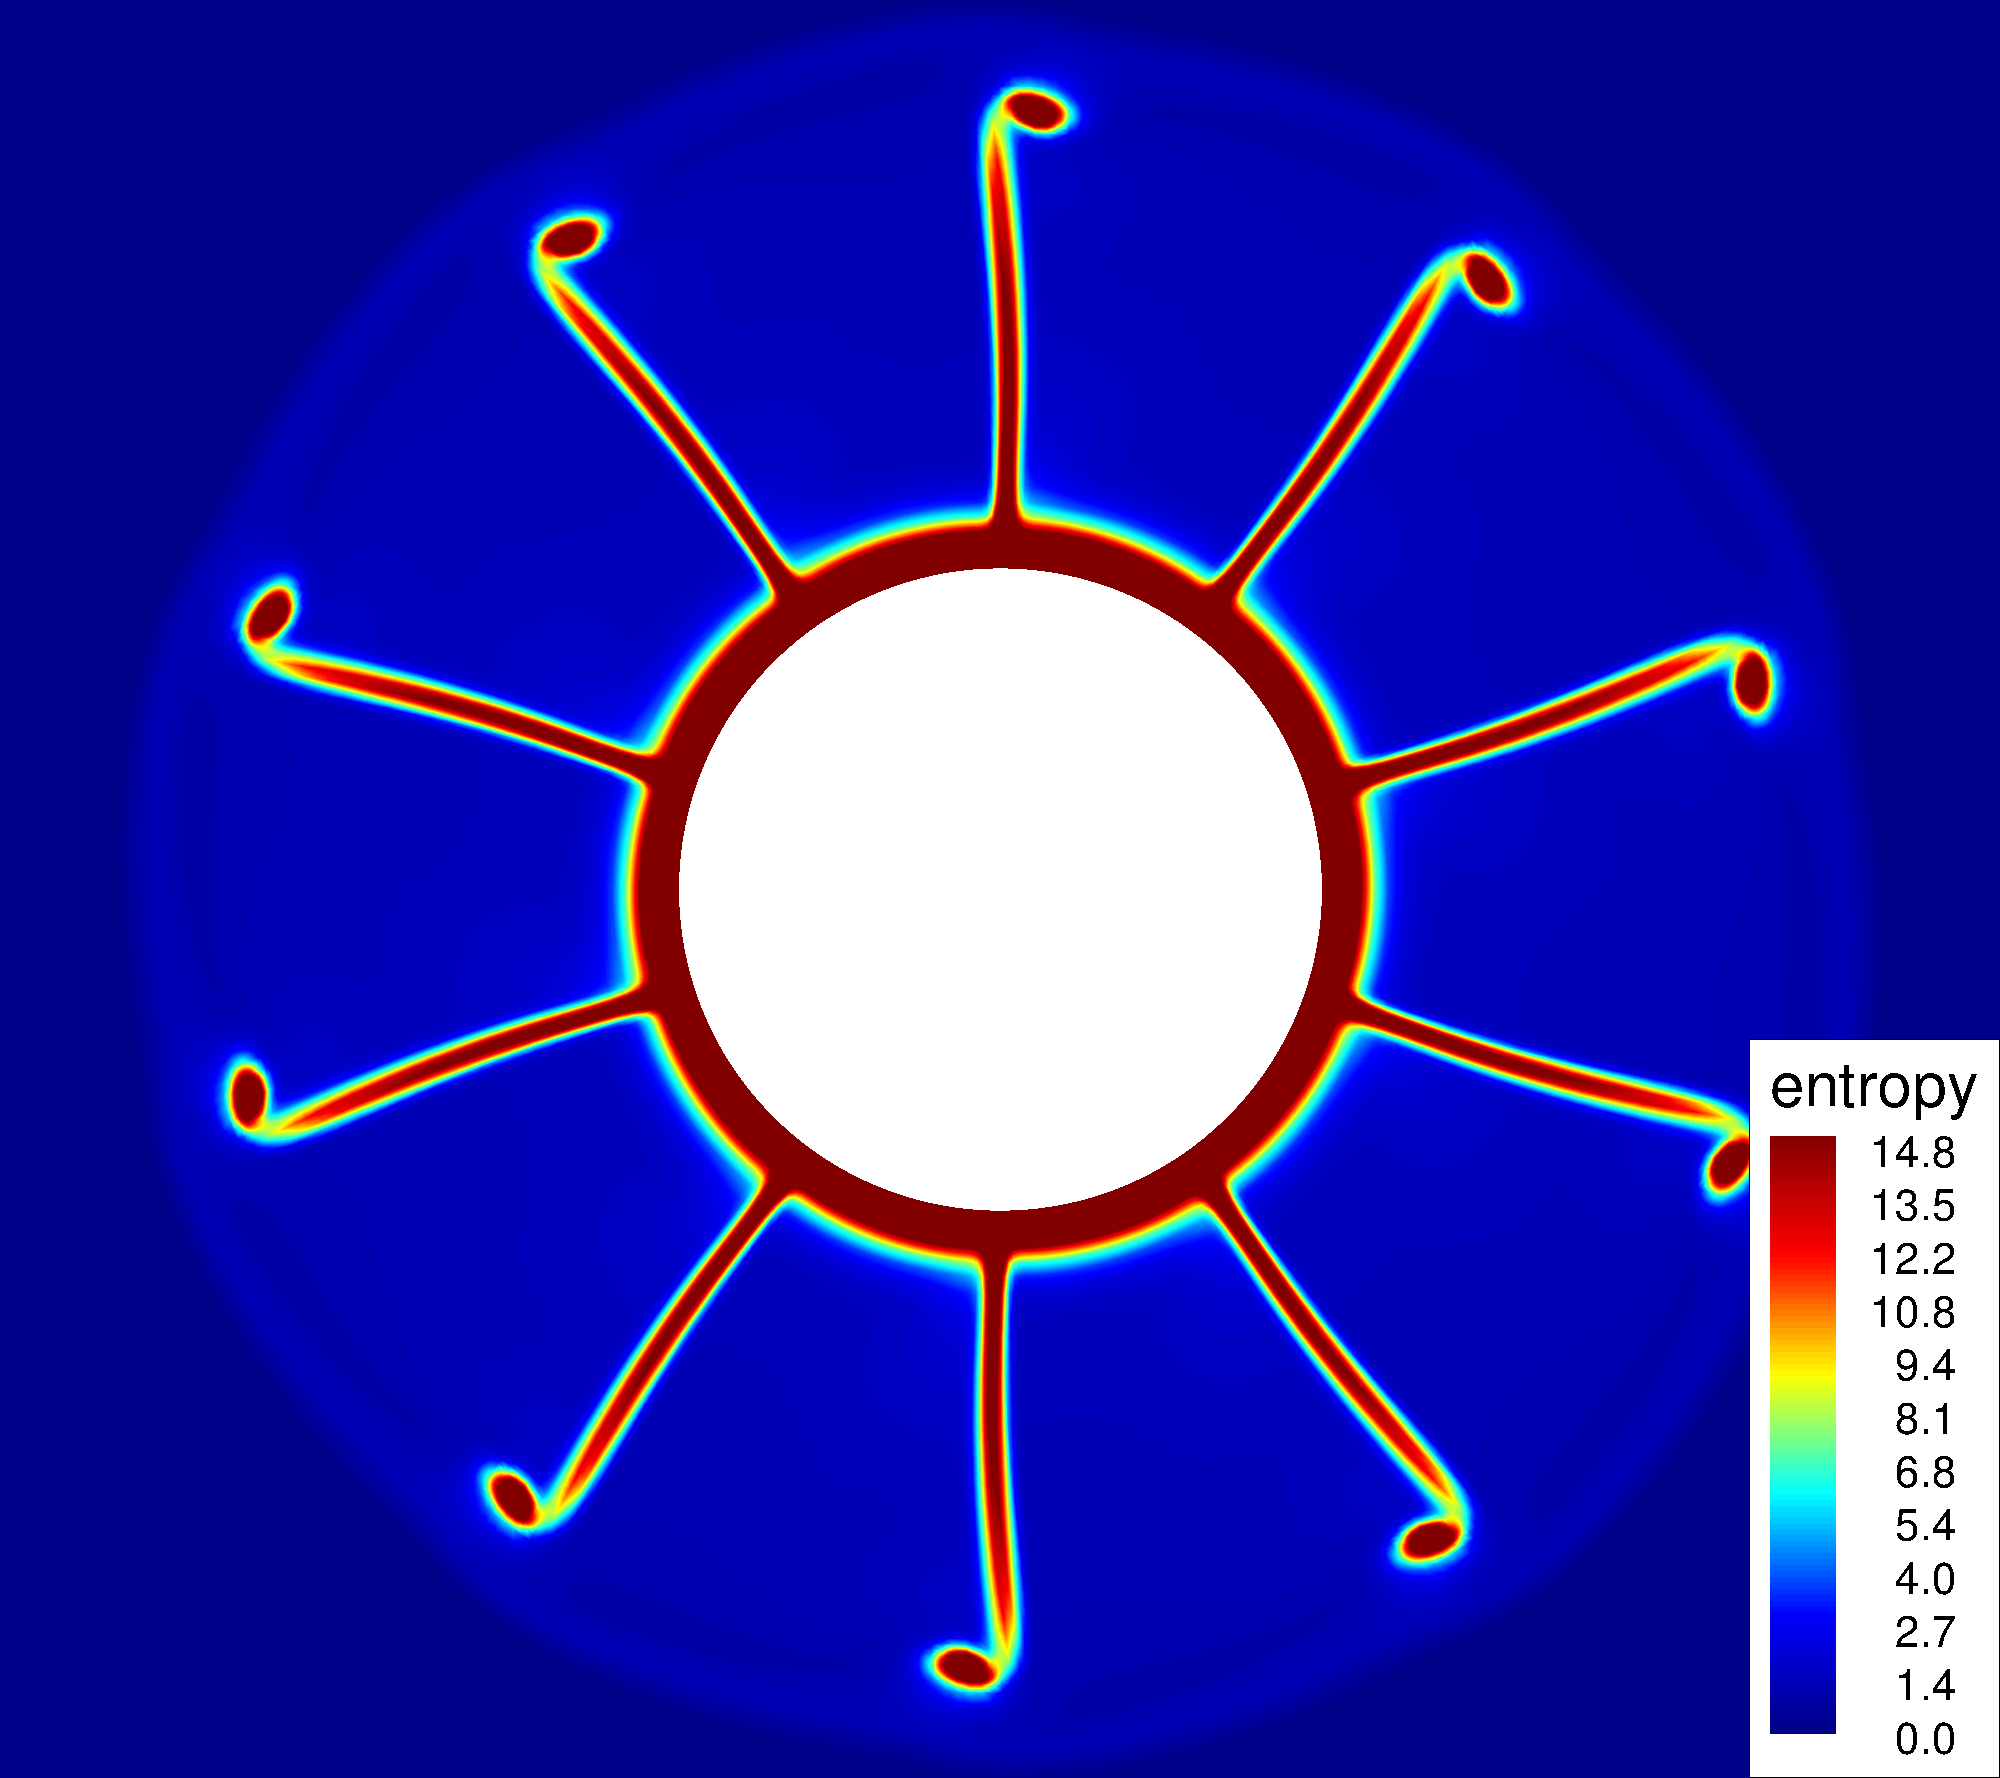
\includegraphics[width=.35\textwidth]{DREAM_HS_RANS_roe2_sa_slice_x_rear_2_entropy.png}
   & 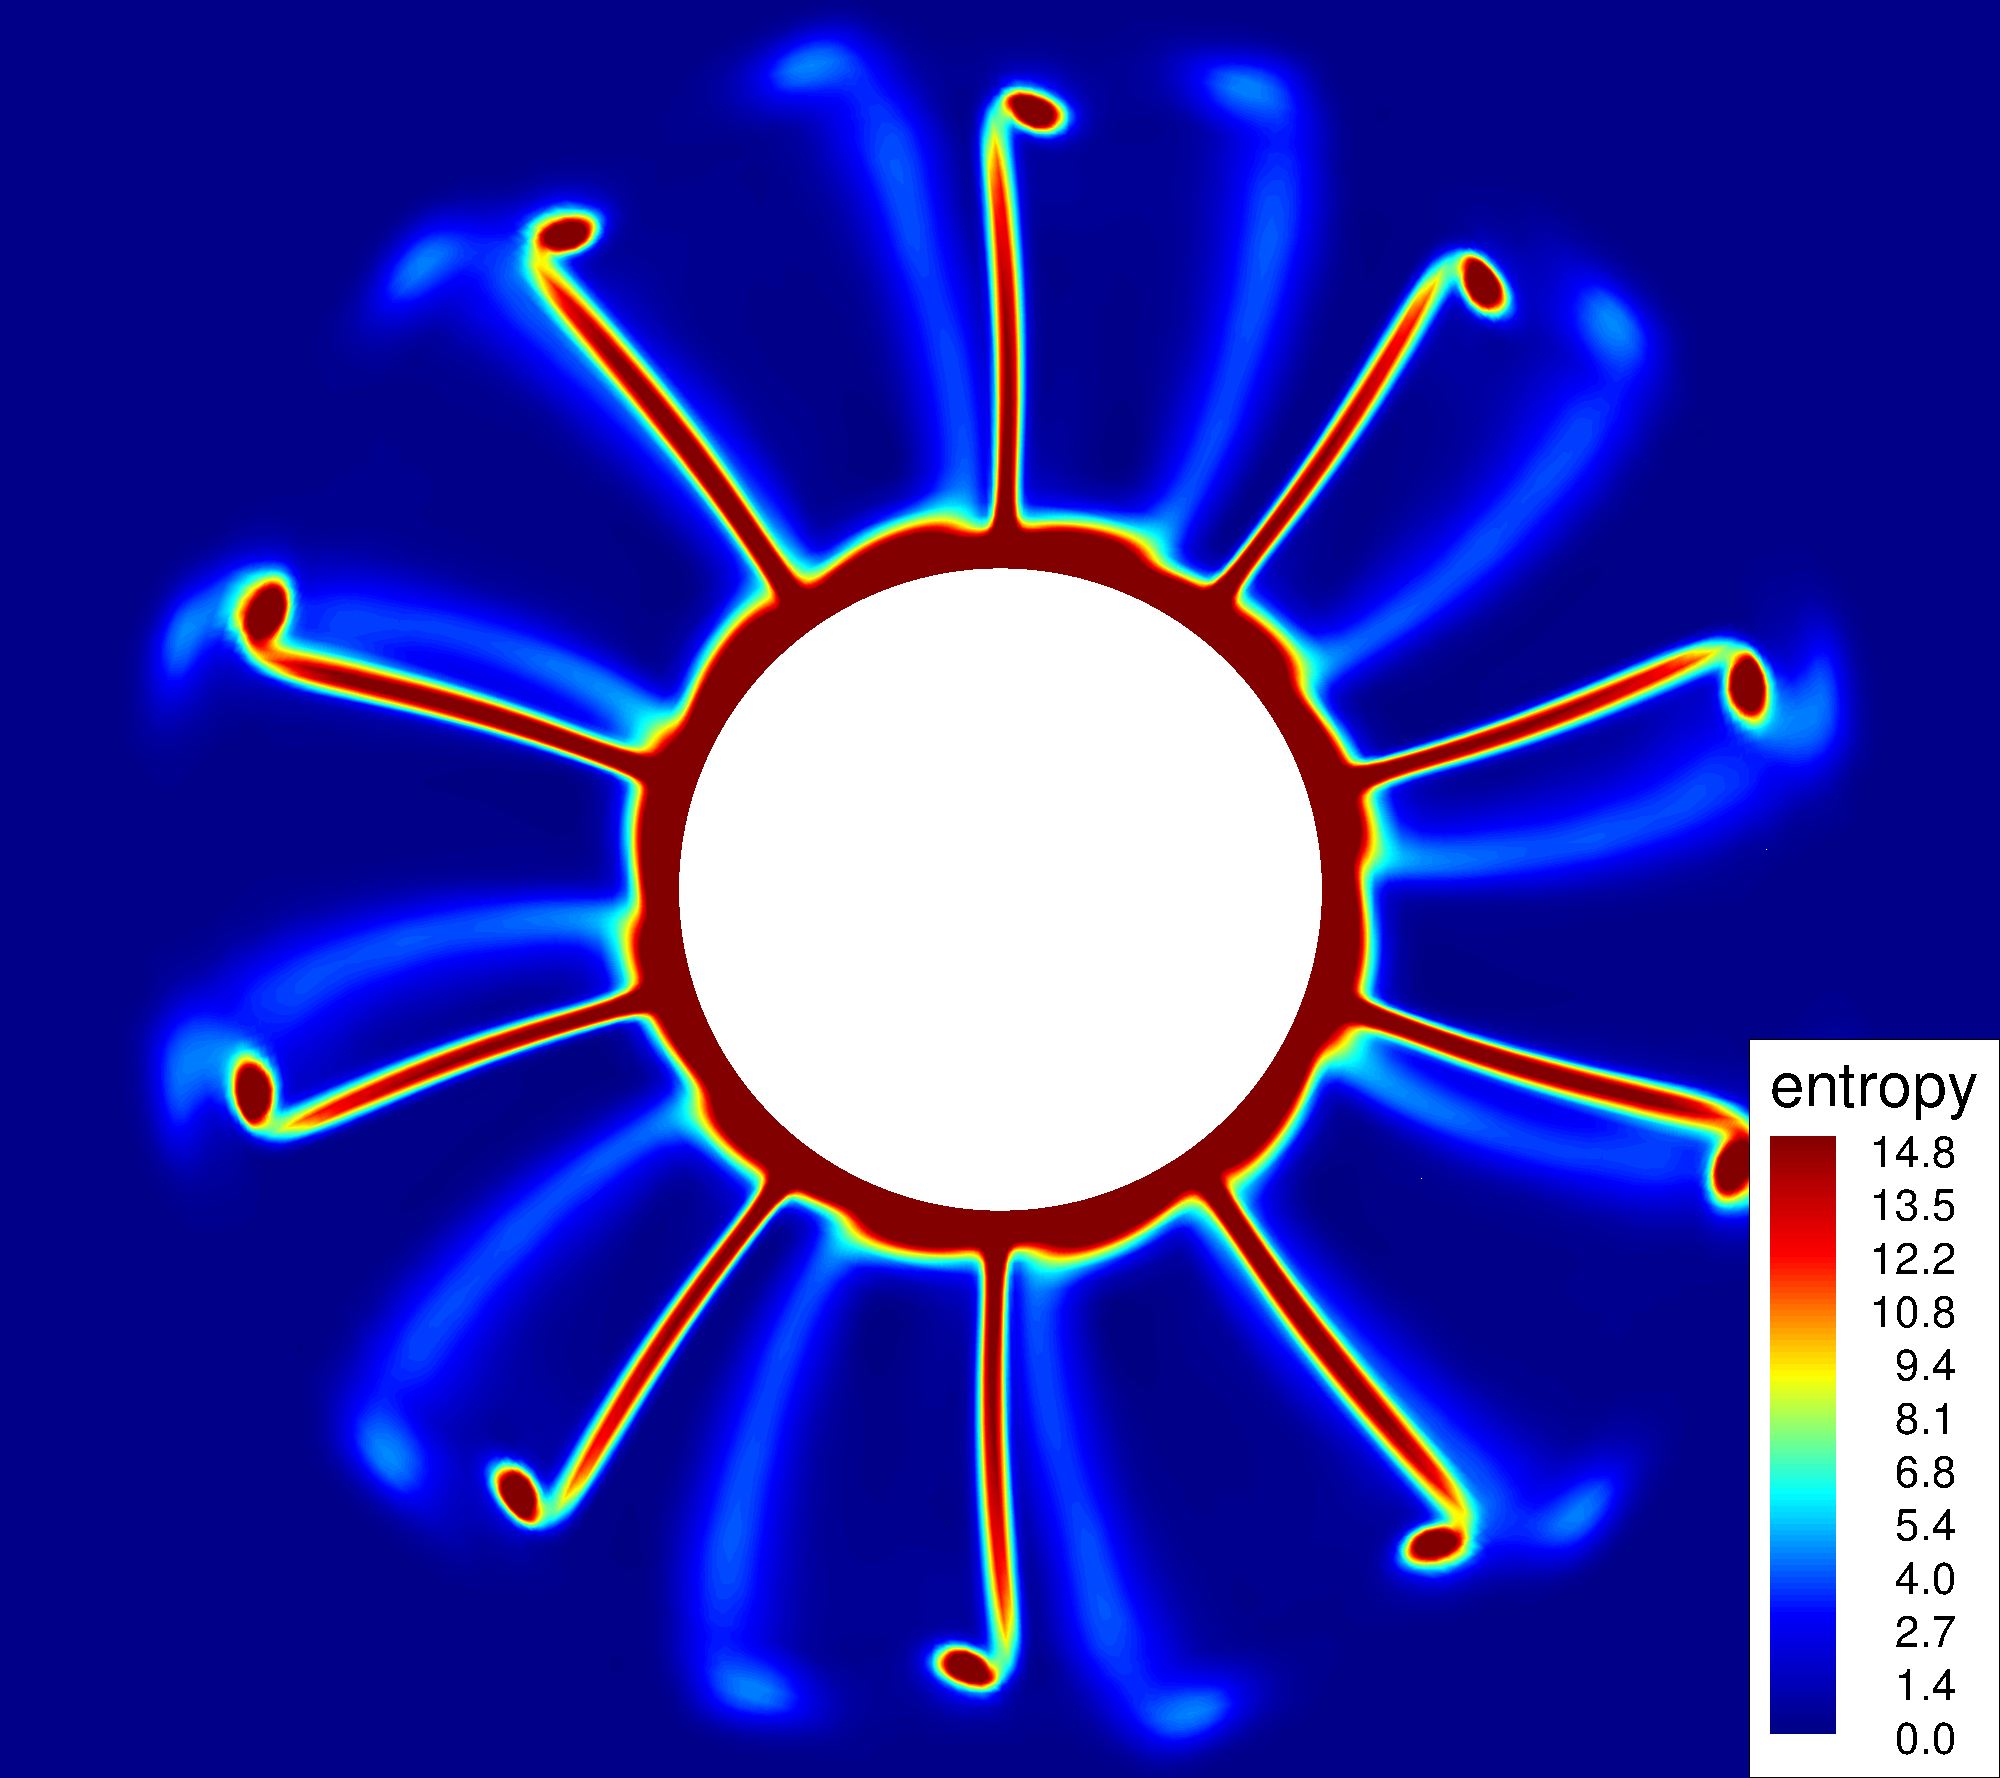
\includegraphics[width=.35\textwidth]{DREAM_HS_TSM_N7_roe2_sa_slice_x_rear_2_entropy.png} \\
 \end{tabular}
 \caption{High-speed isolated configuration: axial cuts of entropy.}
 \label{fig:dream_hs_hb_axial_cut_entropy}
\end{figure}

\subsection{Two-dimensional results: radial cut of harmonic pressure}
\label{sub:dream_hs_hb_radial_cuts}

\begin{figure}[htp]
  \centering
  \includegraphics*[width=0.40\textwidth]{DREAM_HS_TSM_N7_roe2_sa_slice_r_70_ps.png}
  \caption{High-speed isolated configuration: radial cut of the first harmonic of the
  static pressure normalized by the inflow static pressure.}
  \label{fig:dream_hs_hb_radial_cuts}
\end{figure}

\begin{figure}[htp]
  \centering
  \includegraphics*[width=0.40\textwidth]{DREAM_HS_TSM_N7_roe2_sa_slice_r_70_machrel.png}
  \caption{High-speed isolated configuration: radial cut of the first harmonic of the
  relative Mach number.}
  \label{fig:dream_hs_hb_radial_cuts_machrel}
\end{figure}